\chapter{Локализация в открытых квантовых системах}\label{ch:ch1}
Явление локализации Андерсона в пространственно-неоднородных средах \autocite{Anderson1958}, известное уже на протяжении более 60 лет, все ещё приковывает внимание исследователей \autocite{Kramer1993, Evers2008, Esposito2012} и экспериментально наблюдается в различных областях физики \cite{Segev2013, Billy2008, Roati2008, Kondov2011, Jendrzejewski2012}.
Данный феномен является хорошо изученным в контексте невзаимодействующих частиц в когерентном гамильтоновом пределе \autocite{Segev2013, Billy2008, Roati2008, Yedjour2010, Kondov2011, Jendrzejewski2012}.
Но в диссипативных квантовых системах, где есть взаимодействие с окружающей средой, локализация Андерсона изучена не достаточно хорошо \autocite{Breuer2007}.

Физическая интуиция подсказывает, что в открытых квантовых системах диссипация должна оказывать деструктивное виляние на интерференцию волновых пакетов, которая, в свою очередь, является причиной локализации Андерсона.
Ранее проведённые исследования подтвердили, что диссипация разрушает локализацию Андерсона \cite{Gurvitz2000, Nowak2012, Flores1999}. 
Однако недавние результаты проливают свет на гораздо более богатую физику. 
Было продемонстрировано, что даже когда асимптотическое состояние является тривиальным равномерным распределением (состояние с максимальной энтропией), процесс релаксации к данному состоянию проявляет неоднородную динамику и признаки метастабильности \cite{Genway2014}.
В то же время известны случаи, когда диссипативные эффекты могут играть конструктивную роль в приведении квантовых систем в некоторые специфические (чистые и смешанные) состояния \cite{Diehl2008, Kraus2008, Verstraete2009}, в стабилизации квантовых систем в метастабильных состояниях \cite{Valenti2015, Spagnolo2015, Spagnolo2016, Magazz2015, Magazz2016}.
Кроме этого, определённые типы диссипативных эффектов используются для уменьшения потерь и увеличения когерентности в конденсатах Бозе"--~Эйнштейна \cite{Syassen2008, Witthaut2008, Witthaut2011, Kordas2013}.
Первые доказательства того, что локализация Андерсона может существовать, когда в системе есть диссипация, были получены для квазиклассических и классических систем. 
В частности, были получены экспериментальные свидетельства локализации в случайном лазере, за счёт которой уменьшается пространственное перекрытие мод и, в результате, улучшается стабильность лазера \autocite{Stano2012, Liu2014}.
Также было показано, что в классических активных нелинейных системах с беспорядком аттракторы могут демонстрировать локализацию в пространстве («Андерсоновские аттракторы») \cite{Laptyeva2015_1, Laptyeva2015_2}. 

Расширением феномена локализации Андерсона для многочастичных систем является многочастичная локализация (MBL) \cite{Basko2006, Gornyi2005}.
Существует целый спектр определений и квантификаторов этого многогранного явления, нацеленных на выделение специфических свойств систем с многочастичной локализацией.
Среди них можно выделить отсутствие проводимости \autocite{Gornyi2005} (даже в пределе бесконечной температуры \autocite{Basko2006}), медленный логарифмический рост энтропии запутанности при уменьшении параметра взаимодействия между частицами \autocite{Chiara2006, Znidaric2008, Bardarson2012, Serbyn2013_1}, существование обширного набора локальных интегралов движения \autocite{Serbyn2013_2}, и специфические спектральные свойства гамильтонианов \autocite{Oganesyan2007, Serbyn2016}.
Есть также квантификаторы, характеризующие свойства собственных состояний систем с многочастичной локализацией "--- корреляции ближнего действия \autocite{Pal2010}, низкая энтропия запутанности \autocite{Bauer2013, Kjll2014, Khemani2017} и большие флуктуации локальных наблюдаемых \autocite{Bera2015}.

В контексте открытых квантовых систем явление многочастичной локализации все ещё является недостаточно изученным. Влияние диссипации на состояния систем  MBL в больших временных масштабах является очень важным направлением исследования, особенно в контексте недавних экспериментальных работ \autocite{Schreiber2015, Choi2016, Bordia2017, Smith2016}. В связанных теоретических работах \autocite{Levi2016, Fischer2016, Medvedyeva2016} рассматривались открытые системы с дефазирующей диссипацией \autocite{Poletti2013}, из-за которой состояние системы (вне зависимости от силы взаимодействия между частицами и присутствия в системе локализации) со временем приходило в тривиальное асимптотическое состояние с максимальной энтропией.

В данной главе в разделе \cref{sec:ch1/sec1} будет рассмотрен основной предмет исследования "--- открытые квантовые системы, методы их описания и анализа. 
В разделе \cref{sec:ch1/sec2} будет рассмотрен микроскопический метод описания и анализа открытых квантовых систем "--- метод квантовых траекторий.
В разделе \cref{sec:ch1/sec3} описывается открытая модель Андерсона, в которой впервые были найдены следы локализации в открытых квантовых системах.
В разделе \cref{sec:ch1/sec4} подробно излагаются признаки локализации, описываются результаты численных экспериментов и теоретические выкладки объясняющие природу локализации в открытых квантовых системах. 

\section{Описание открытых квантовых систем}\label{sec:ch1/sec1}

Наиболее общепринятым способом описания динамики открытых квантовых систем, то есть систем, взаимодействующих с окружающей средой, является уравнение Линдблада (Горини"--~Коссаковского"--~Сударшана"--~Линдблада, GKSL equation) \cite{Gorini1976, Lindblad1976, Chruciski2017} для матрицы плотности \(\rho (t)\):

\begin{equation}
\label{eq:GKSL_base}
\begin{gathered}
\frac{\partial}{\partial t} \rho (t) = \mathcal{L}(\rho(t), t) = -i \left[ H(t), \rho(t) \right] + \sum_{k=1}^{K} \gamma_{k}(t) \mathcal{D}_k(t), \\
\mathcal{D}_k(t) =  V_k(t) \rho(t) V_k^\dagger(t) - \frac{1}{2} \left\lbrace V_k^\dagger(t) V_k(t), \rho(t) \right\rbrace ,
\end{gathered}
\end{equation}
где первое слагаемое в правой части первого уравнения является унитарной частью, которая отвечает за когерентную эволюцию системы с гамильтонианом \(H(t)\), а второе слагаемое в правой части "--- диссипативная часть, отвечающая за взаимодействие с окружающей средой. Символы \(\left[ \cdot, \cdot \right]\) и  \(\left\lbrace \cdot, \cdot \right\rbrace\) обозначают коммутатор и антикоммутатор соответственно. Взаимодействие с окружающей средой в системе осуществляется через \(K\) каналов диссипации, каждый из которых характеризуется скоростью диссипации \(\gamma_{k}(t)\) и непосредственно диссипативным оператором (диссипатором) \(V_k(t)\).  
Данное представление активно используется при описании процессов в квантовой оптике \cite{Carmichael1993}, оптомеханических системах \cite{Aspelmeyer2014}, квантовой электродинамике \cite{Jin2013, Fitzpatrick2017} и физике ультрахолодных атомов \cite{Diehl2008, Marcuzzi2014}.

Уравнение \cref{eq:GKSL_base} можно представить в виде однородной системы линейных дифференциальных уравнений с переменными коэффициентами:
\begin{equation}
\label{eq:GKSL_lindbladian}
\begin{gathered}
\frac{\partial}{\partial t} \rho (t) = L(t)\rho(t), \\
L(t) = -i \left( \idmtx \otimes H(t) - H^\top(t) \otimes \idmtx \right) + \\
+ \sum_{k=1}^{K} \gamma_{k}(t) \cdot \idmtx \otimes V_k(t) \cdot \overline{V_k}(t) \otimes \idmtx - \\ 
- \sum_{k=1}^{K} \frac{1}{2} \gamma_{k}(t) \cdot V_k^\top(t) \overline{V_k}(t) \otimes \idmtx - \\
- \sum_{k=1}^{K} \frac{1}{2} \gamma_{k}(t) \cdot \idmtx \otimes V_k^\dagger(t) V_k(t),
\end{gathered}
\end{equation}
где \(\idmtx\) "--- единичная матрица размерности \(N \times N\) (\(N\) - число состояний в квантовой системе). 
Матрица плотности (размерности \(N \times N\)) разворачивается по строкам в виде супервектора (размерности \(N^2 \times 1\)).
Матрица оператора Линдблада (линдбладиан) \(L(t)\) имеет размерность \(N^2 \times N^2\).

В случае, если линдбладиан не зависит от времени, уравнение \cref{eq:GKSL_lindbladian} имеет единственное асимптотические состояние равновесия (матрицу плотности) \(\rho^A\) \cite{book2007}.
Данная матрица плотности является нулевым собственным состоянием линдбладиана "--- собственным вектором, который соответствует нулевому собственному числу и развернут в виде матрицы \cite{Albert2014, Albert2016}.

В случае, если линдбладиан является периодическим во времени \(\mathcal{L}(\rho,t + T) = \mathcal{L}(\rho,t)\) с периодом \(T\), то, согласно теории Флоке \cite{Meyer1977}, асимптотическая матрица плотности также является периодической с тем же периодом: \(\rho^A(t + T) = \rho^A(t)\) \cite{Hartmann2017}.

Основная вычислительная задача, решаемая при исследовании открытых квантовых систем "--- отыскание асимптотической матрицы плотности в стационарном и периодически модулируемом случае. 
Есть три общепринятых пути ее вычисления:
\begin{enumerate}[beginpenalty=10000] % https://tex.stackexchange.com/a/476052/104425
	\item Спектральные методы (полная или частичная диагонализация линдбладиана и различные виды итерационных алгоритмов \cite{Nation2015, eigenweb, Hernandez2005});
	\item Численное интегрирование уравнения \cref{eq:GKSL_lindbladian} при помощи схем высоких порядков \cite{Lambert1991};
	\item Метод квантовых траекторий \cite{Dum1992, Molmer1993, Plenio1998, Daley2014}, позволяющий свести задачу численного решения уравнения \cref{eq:GKSL_lindbladian} к задаче статистического семплирования отдельных квантовых траекторий, уравнения для которых содержат на порядок меньшее количество состояний.
	Описание метода квантовых траекторий приведено в разделе \cref{sec:ch1/sec2}.
\end{enumerate}


\section{Метод квантовых траекторий}\label{sec:ch1/sec2}
Для получения численного решения уравнения \cref{eq:GKSL_lindbladian} в заданный момент времени \(t^F\) методом квантовых траекторий (также известным как метод Монте-Карло для волновых функций \cite{Molmer1993}) необходимо сначала вычислить эффективный неэрмитовый гамильтониан:
\begin{equation}
\label{eq:H_nonhermit}
\begin{gathered}
\tilde{H}(t) = H(t) - \frac{i}{2} \sum_{k=1}^{K} V_k^\dagger(t) V_k(t),
\end{gathered}
\end{equation}
и рассмотреть эволюцию каждой отдельной квантовой траектории с данным гамильтонианом:
\begin{equation}
\label{eq:schrodinger}
\begin{gathered}
i \frac{\partial}{\partial t} \psi_j(t) = \tilde{H}(t) \psi_j(t)
\end{gathered}
\end{equation}
Здесь волновая функция \(\psi_j(t)\) описывает состояние \(j\)-ой квантовой траектории в момент времени \(t\). Эволюция волновой функции будет прерываться случайными квантовыми скачками, индуцированными диссипативными операторами \(V_k(t)\). Если необходимо достижение асимптотического режима, нужно выбирать время \(t^F\) достаточным для окончания всех процессов релаксации системы.

Полное описание метода квантовых траекторий выглядит следующим образом \cite{Volokitin2017}:

\IncMargin{1em}
\begin{algorithm}
	\SetAlgoLined
	\SetKwProg{Fn}{Function}{:}{}
	\SetKwFunction{none}{None}
	
	Инициализация неэрмитового гамильтониана \(\tilde{H}(t)\) из уравнения \cref{eq:H_nonhermit}\;
	Инициализация стартового значения \( \left| \psi^{init} \right\rangle \) для \(M_r\) траекторий\;
	\For{\(j\leftarrow 1\) \KwTo \(M_r\)}
	{
		Инициализация стартового времени для \(j\)-ой траектории: \(t_j\leftarrow0\)\;
		\While{\(t_j < t^F\)}{
			Генерация случайной величины \(\eta\), равномерно распределённой в интревале \(\left[0; 1\right] \)\;
			Численное пропагирование состояния волновой функции \( \left| \psi_j (t) \right\rangle \) на время, необходимое для убывания квадрата нормы волновой функции до значения \(\eta\): \(\norm{\left| \psi_j(t_j) \right\rangle}^2 = \eta\)\;
			Нормализация волновой функции: \( \left| \psi_j (t_j) \right\rangle \leftarrow \frac{\left| \psi_j (t_j) \right\rangle}{\norm{\left| \psi_j(t_j) \right\rangle}} \)\;
			Осуществление квантового скачка через случайно выбранный диссипативный оператор \(V_k(t_j)\) с вероятностью \(p_k\leftarrow\gamma_k(t_j) \frac{\norm{ V_k(t_j) \left| \psi_j(t_j) \right\rangle}^2}{\sum_{l=1}^{K} \norm{ V_l(t_j) \left| \psi_j(t_j) \right\rangle}^2}\)\;
			Трансформация волновой функции с учетом выбранного канала диссипации: \( \left| \psi_j (t_j) \right\rangle \leftarrow \frac{ V_k(t_j) \left| \psi_j (t_j) \right\rangle}{\norm{V_k(t_j) \left| \psi_j(t_j) \right\rangle}}\)\;
		}
	}
	Вычисление матрицы плотности в момент времени \(t^F\) при помощи \(M_r\) квантовых траекторий: \(\rho_{M_r}(t^F) \leftarrow \frac{1}{M_r}\sum_{j=1}^{M_r} \left| \psi_j (t^F) \left\rangle \right\langle \psi_j (t^F)  \right| \)\;
	
	\caption{Метод квантовых траекторий}
	\label{alg:qt_main}
\end{algorithm}
\DecMargin{1em}

Формально, в пределе \(M_r \rightarrow \infty\) матрица плотности сходится к решению уравнения \cref{eq:GKSL_lindbladian} в момент времени \(t^F\) для заданной начальной матрицы плотности \( \rho^{init} = \left| \psi^{init} \left\rangle \right\langle \psi^{init} \right|\) \cite{Breuer2007, Dum1992}.

Промежуток времени между двумя последовательными квантовыми скачками заранее не известен и его длительность можно вычислить только при непосредственном пропагировании квантовой траектории. 
При пропагации траектории необходимо контролировать убывающий квадрат нормы волновой функции и определить момент времени, когда он станет равен случайному значению \(\eta\).

В случае, если система является периодически модулируемой, и функция модуляции является непрерывно зависящей от времени, то в данном случае возможно применение классических методов численного интегрирования \cite{Lambert1991} с достаточно маленьким шагом \cite{Breuer2007}, а также специальные схемы для стохастических дифференциальных уравнений \cite{Cao2003}.

\IncMargin{1em}
\begin{algorithm}
	\SetAlgoLined
	\SetKwProg{Fn}{Function}{:}{}
	\SetKwFunction{prop}{Propagation}
	\SetKwFunction{jump}{Jump}
	\Fn{\prop{\(\left| \psi_j (t) \right\rangle\), \(t\), \(\eta\), \(d\)}}{
		
		\For{\(s_d\leftarrow 1\) \KwTo \(2\)}{
			\( | \tilde{\psi}_j(t) \rangle \leftarrow \mathcal{P}_{d} \left| \psi_j(t) \right\rangle \)\; \label{alg:mvmult}
			\uIf{d = D}{
				\uIf{\( \norm{| \tilde{\psi}_j(t) \rangle}^2 < \eta\)}{
					\jump{\(| \tilde{\psi}_j(t) \rangle\)}\;
					\(\eta \leftarrow \) новое случайносгенерированное число\;
				}
				\(\left| \psi_j(t) \right\rangle \leftarrow | \tilde{\psi}_j(t) \rangle\)\;
			}
			\Else{
				\uIf{\( \norm{| \tilde{\psi}_j(t) \rangle}^2 < \eta\)}{
					\prop{\(\left| \psi_j (t) \right\rangle\), \(t\), \(\eta\), \(d + 1\)}\;
					\(t \leftarrow t - \tau_d\)\;
				}
				\Else{
					\(\left| \psi_j(t) \right\rangle \leftarrow | \tilde{\psi}_j(t) \rangle\)\;
				}	
			}
			
			\(t \leftarrow t + \tau_d\)\;
		}
		\(s_d \leftarrow 0\)\;
	}
	\caption{Функция прогагации квантовой траектории на заданной глубине \(d\)}
	\label{alg:qt_recursive}
\end{algorithm}
\DecMargin{1em}

В случае, если система является автономной или периодической с кусочно"--~постоянной функцией модуляции, то применима специальная схема на основе экспоненциальных пропагаторов \cite{Volokitin2017}.
Пропагирование на любой временной интервал \(\tau\), в рамках которого эффективный гамильтониан \(\tilde{H}\) остаётся постоянным, может быть выполнено при помощи специального пропагирующего оператора (пропагатора):
\begin{equation}
\label{eq:propagator}
\begin{gathered}
\mathcal{P}_{\tau} = e^{-i \tilde{H} \tau},
\end{gathered}
\end{equation}
где \(e\) "--- функция матричной экспоненты \cite{Moler2003}. Для отыскания времени квантового прыжка использовался эффективный метод бисекции \cite{Knuth1997} c максимальной глубиной \(D\). 
Для реализации данного метода предложена рекурсивная функция осуществляющая пропагацию за данной глубине бисекции \(d\) (алгоритм \ref{alg:qt_recursive}), использующая функцию осуществления квантового скачка (алгоритм \ref{alg:qt_jump}).

\IncMargin{1em}
\begin{algorithm}
	\SetAlgoLined
	\SetKwProg{Fn}{Function}{:}{}
	\SetKwFunction{jump}{Jump}
	\Fn{\jump{\(\left| \psi_j (t) \right\rangle\)}}{
		
		Нормализация волновой функции: \( \left| \psi_j (t) \right\rangle \leftarrow \frac{\left| \psi_j (t) \right\rangle}{\norm{\left| \psi_j(t) \right\rangle}} \)\;
		Осуществление квантового скачка через случайно выбранный диссипативный оператор \(V_k(t)\) с вероятностью \(p_k\leftarrow\gamma_k(t) \frac{\norm{ V_k(t) \left| \psi_j(t) \right\rangle}^2}{\sum_{l=1}^{K} \norm{ V_l(t) \left| \psi_j(t_j) \right\rangle}^2}\)\;
		Трансформация волновой функции с учетом выбранного канала диссипации: \( \left| \psi_j (t) \right\rangle \leftarrow \frac{ V_k(t) \left| \psi_j (t) \right\rangle}{\norm{V_k(t) \left| \psi_j(t) \right\rangle}}\)\;
	}
	\caption{Функция квантового скачка}
	\label{alg:qt_jump}
\end{algorithm}
\DecMargin{1em}

Результирующий алгоритм пропагации квантовой траектории методом бисекции с независимым от времени эффективным гамильтонианом \(\tilde{H}\) на время \(\tau\) выглядит следующим образом:

\IncMargin{1em}
\begin{algorithm}
	\SetAlgoLined
	\SetKwProg{Fn}{Function}{:}{}
	\SetKwFunction{prop}{Propagation}
	
	Инициализация стартовой глубины бисекции: \(d=1\)\;
	Инициализация шага пропагирования для каждой глубины бисекции: \(\tau_d = \frac{\tau}{2^{d-1}}\) для \(d=1 \ldots D\)\;
	Инициализация матриц пропагаторов \cref{eq:propagator} для каждой глубины бисекции: \(\mathcal{P}_{d} = e^{-i \tilde{H} \tau_d}\) для \(d=1 \ldots D\)\;
	\prop{\(\left| \psi_j (t) \right\rangle\), \(t\), \(\eta\), \(d\)}\;

	\caption{Алгоритм пропагации квантовой траектории методом бисекции на время \(\tau\)}
	\label{alg:qt_prop}
\end{algorithm}
\DecMargin{1em}

В случае, если неэрмитовый гамильтониан непрерывно зависит от времени, то можно использовать аналогичные алгоритмы пропагации, основанные на схемах численного интегрирования высоких порядков.

C вычислительной точки зрения, самая ресурсоемкая операция "--- умножение матрицы \(\mathcal{P}_{d}\) на вектор \(\left| \psi_j(t) \right\rangle \) в строке \ref{alg:mvmult} алгоритма \ref{alg:qt_recursive}. С целью ускорения вычислений, в программной реализации на языке C++ использовалась соответствующая функция из библиотеки Eigen \cite{eigenweb}.

\section{Открытая модель Андерсона}\label{sec:ch1/sec3}
Открытая одночастичная модель Андерсона описывается уравнением Линдблада \cref{eq:GKSL_base, eq:GKSL_lindbladian} c независящим от времени гамильтонианом \cite{Anderson1958}:
\begin{equation}
\label{eq:anderson_H}
\begin{gathered}
H = \sum_{n} \varepsilon_n b^\dagger_n b_n - \left(b^\dagger_n b_{n+1} + b^\dagger_{n+1} b_{n}\right),
\end{gathered}
\end{equation}
где \(\varepsilon_n \in \left[-\frac{W}{2}, \frac{W}{2}\right]\) "--- случайные некореллированые значения энергий на сайте \(n\), \(W\) "--- сила пространственного беспорядка, \(b_n\) и \(b^\dagger_n\) "--- операторы рождения и уничтожения бозона на сайте \(n\). Известно, что собственные значения гамильтониана для этой модели находятся в следующем интервале:
\begin{equation}
\label{eq:anderson_evals}
\begin{gathered}
\lambda_\nu \in \left[-2-\frac{W}{2}, 2+\frac{W}{2}\right],
\end{gathered}
\end{equation}
а соответствующие им собственные вектора \(A_\nu\) являются экспоненциально локализованными в пространстве с длиной локализации \cite{Thouless1983}:
\begin{equation}
\label{eq:anderson_loc_length}
\begin{gathered}
\xi_{\lambda} \approx \frac{24\left(4-\lambda^2\right)}{W^2},
\end{gathered}
\end{equation}
c небольшими поправками на границах спектра \cite{derrida1984lyapounov}.

Асимптотическая матрица плотности \(\rho^A\) формируется не только гамильтонианом, но и окружением открытой квантовой системы "--- диссипативными операторами. В простейшем случае, когда все диссипативные операторы эрмитовы (\(V_k \equiv V^\dagger_k \)), асимптотическая матрица плотности будет иметь тривиальный вид: \(\rho^A=\frac{\idmtx}{N}\), характеризующий состояние системы с максимальной энтропией (\(N\) "--- размерность системы). 
Такой тип диссипации не приводит к локализации, но для полного и всестороннего анализа такие диссипаторы тоже будут использоваться в данной работе:
\begin{equation}
\label{eq:anderson_diss_dephase}
\begin{gathered}
V_k = b^\dagger_k b_k.
\end{gathered}
\end{equation}
Данный вид диссипаторов активно используется при изучении релаксационных процессов в одночастичных \cite{Genway2014} и многочастичных \cite{Fischer2016, Levi2016, Everest2017, Lazarides2017, Lschen2017} открытых квантовых системах.

С другой стороны, формально существует бесконечно много вариантов неэрмитовых диссипаторов \(V_k\), которые гарантируют локализованное асимптотическое состояние в виде \(\rho^A = | \phi_n \rangle \langle \phi_n |\), где \(| \phi_n \rangle\) "--- \(n\)-oе собственное состояние гамильтониана \(H\) \cref{eq:anderson_H}. 
Чтобы это выполнялось, собственное состояние \(| \phi_n \rangle\) должно быть так называемым «тёмным» состоянием для всех диссипативных операторов, то есть должно выполняться условие \(V_k | \phi_n \rangle = 0\) для всех \(k=1 \ldots K\) \cite{Diehl2008, Kraus2008}. 
Однако, на практике для этого необходимо априорное знание состояния \(| \phi_n \rangle\) и создание физически нереализуемых диссипативных операторов.
В данной работе будут применяться физически реализуемые неэмитовые диссипаторы, которые активно использующиеся при изучении открытых квантовых систем \cite{Diehl2008, Kraus2008, Bardyn2013, Barreiro2010, Kienzler2014, Vorberg2013}:
\begin{equation}
\label{eq:anderson_diss_local}
\begin{gathered}
V_k = \left( b^\dagger_k + e^{i \alpha} b^\dagger_{k+l}\right) \left( b_k - e^{-i \alpha} b_{k+l} \right),
\end{gathered}
\end{equation}
где \(\alpha\) "--- фаза диссипатора, а \(l\) определяет индекс соседнего сайта, на который воздействует данный диссипатор. 
В случае, когда \(\alpha = 0\), диссипативный оператор синхронизует динамику на \(k\)-ом и \((k+l)\)-ом сайте, за счёт рециркуляции антисимметричных противофазных состояний в симметричные и синфазные. 
Данный тип диссипаторов с \(l=1\) был впервые представлен в работах \cite{Diehl2008, Kraus2008}.
Экспериментальная реализация цепочки Бозе"--~Хаббарда с сайтами, соединёнными диссипаторами такого вида, обсуждается в работе \cite{Marcos2012}, за счёт использования квантовых резонаторов, соединённых сверхпроводящими кубитами.
Фаза диссипатора \(\alpha\) в данной установке может варьироваться относительным положением кубита.

\section{Локализация в открытых квантовых системах}\label{sec:ch1/sec4}

В открытой квантовой модели Андерсона \cref{eq:GKSL_lindbladian, eq:anderson_H} c неэрмитовыми диссипаторами \cref{eq:anderson_diss_local} зафиксируем граничные условия \(\rho_0 = \rho_{N+1} = 0\) (\(N = 100\) "--- число состояний в системе) и проанализируем асимптотическую матрицу плотности \(\rho^A\), которая является единственным состоянием равновесия в уравнении \cref{eq:GKSL_lindbladian} \cite{book2007, Albert2014}. Коэффициенты скорости диссипации "--- константные значения \(\gamma_k = 0.1\) для всех \(k\).
Так как в данной модели линдбладиан не зависит от времени, асимптитическую матрицу плотности можно искать путем вычисления нулевого собственного вектора линдбладиана \(L\) \cref{eq:GKSL_lindbladian} при помощи библиотеки Eigen \cite{eigenweb}.

\begin{figure}[ht]
	\centerfloat{
		\hfill
		\subcaptionbox[List-of-Figures entry]{\label{fig:anderson_rho_loc-1}}{%
			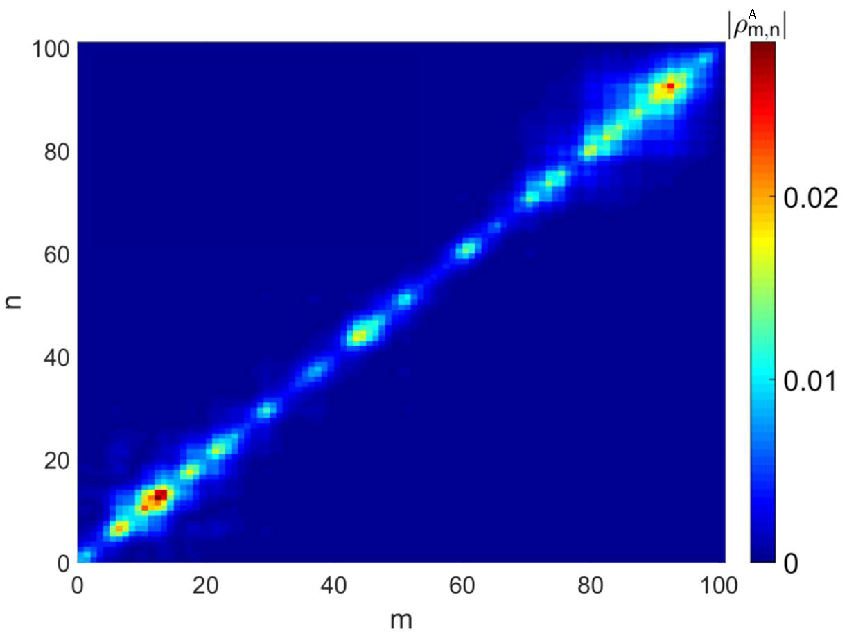
\includegraphics[width=0.5\linewidth]{anderson_rho_loc_1}}
		\hfill
		\subcaptionbox{\label{fig:anderson_rho_loc-2}}{%
			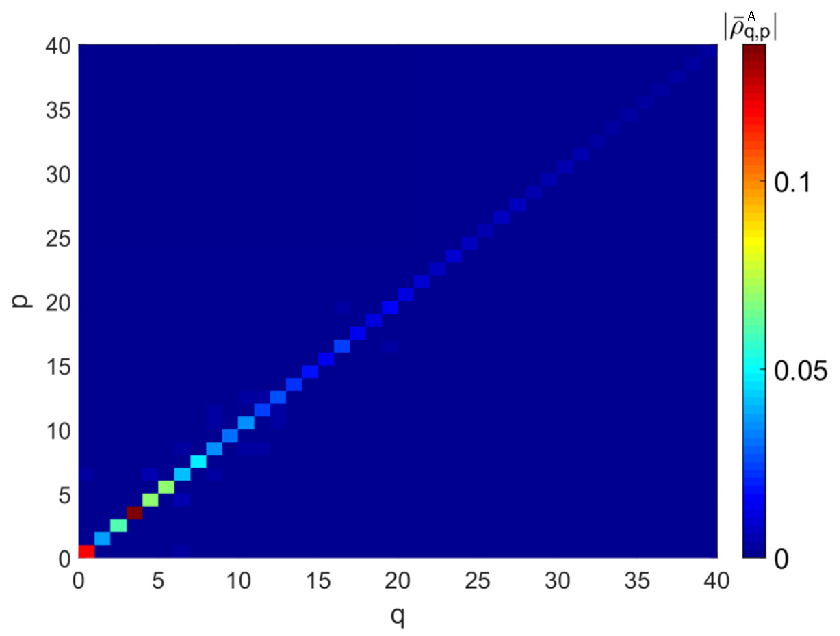
\includegraphics[width=0.5\linewidth]{anderson_rho_loc_2}}
		\hfill
	}
	\legend{}
	\caption[Этот текст попадает в названия рисунков в списке рисунков]
	{
		Абсолютные значения асимптотической матрицы плотности \(\rho^A\) в исходном базисе (a) и в базисе собственных состояний модели Андерсона (б) для единичной реализации беспорядка. Использовались неэрмитовые диссипаторы \cref{eq:anderson_diss_local} c параметрами \(\alpha=0\) и \(l=1\). Сила пространственного беспорядка \(W=1\).
	}
	\label{fig:anderson_rho_loc}
\end{figure}

Зафиксируем параметры диссипаторов \(\alpha=0\) и \(l=1\) в формуле \cref{eq:anderson_diss_local} (синфазная диссипация на соседних сайтах решётки). В этом случае асимптотическая матрица плотности \(\rho^A\) имеет пятнистую структуру с несколькими яркими областями локализации, как показано на рисунке~\cref{fig:anderson_rho_loc-1}.
Рассмотрим асимптотическую матрицу плотности \(\rho^A\) в базисе собственных состояний модели Андерсона:
\begin{equation}
\label{eq:anderson_rho_in_eigen_basis}
\begin{gathered}
\bar{\rho}^A = \mathcal{A}^\dagger \rho^A \mathcal{A},
\end{gathered}
\end{equation}
где \(\mathcal{A} = \left(A_1 \ldots A_\nu \ldots A_N \right) \) "--- матрица собственных векторов гамильтониана \cref{eq:anderson_H}. В данном представлении матрица плотности \(\bar{\rho}^A\) является практически диагональной, с большим преобладанием значений из нижней части спектра, как показано на рисунке~\cref{fig:anderson_rho_loc-2}.

Для аналитического подтверждения данного наблюдения перепишем уравнение \cref{eq:GKSL_base} в базисе собственных состояний модели Андерсона \cref{eq:anderson_rho_in_eigen_basis}, пренебрегая недиагональными элементами матрицы плотности. В таком приближении эволюция диагональных элементов определяется только диссипативными членами:
\begin{equation}
\label{eq:anderson_diag_mod_1}
\begin{gathered}
\dot{\bar{\rho}}_{p,p} = \gamma \left( \sum_q I_{p,q}\bar{\rho}_{q,q} - \bar{\rho}_{p,p} \sum_q I_{q,p} \right),
\end{gathered}
\end{equation}
где коэффициенты перекрытий \(I_{p,q}\) представляются следующим образом через диссипативные операторы в базисе собственных состояний модели Андерсона (\(\bar{V}_k = \mathcal{A}^\dagger V_k \mathcal{A}\)):
\begin{equation}
\label{eq:anderson_diag_mod_2}
\begin{gathered}
I_{p,q} = \sum_k \left| \left(\bar{V}_k\right)_{q,p} \right|^2 = \sum_k \left(\mathcal{A}_{p, k+l} + e^{i \alpha} \mathcal{A}_{p, k} \right)^2  \left(\mathcal{A}_{q, k+l} - e^{-i \alpha} \mathcal{A}_{q, k} \right)^2.
\end{gathered}
\end{equation}
Система линейных дифференциальных уравнений \cref{eq:anderson_diag_mod_1} имеет единственное устойчивое состояние равновесия. Для его поиска, приравняем правую часть уравнения к \(0\), введём переобозначение:
\begin{equation}
\label{eq:anderson_diag_mod_3}
\begin{gathered}
I^{\pm}_{p,k} = \left(\mathcal{A}_{p, k+l} \pm e^{\pm i \alpha} \mathcal{A}_{p, k} \right)^2 ,
\end{gathered}
\end{equation}
и получим итоговое выражение для асимптотического состояния равновесия:
\begin{equation}
\label{eq:anderson_diag_mod_4}
\begin{gathered}
\bar{\rho}^A_{p,p} = \frac{\sum_q I_{p,q}\bar{\rho}^A_{q,q}}{\sum_q I_{q,p}} = \frac{\sum_q \sum_k I^{+}_{p,k} I^{-}_{q,k} \bar{\rho}^A_{q,q}}{\sum_q \sum_k I^{+}_{q,k}  I^{-}_{p,k}} = \frac{\sum_k I^{+}_{p,k} \sum_q I^{-}_{q,k} \bar{\rho}^A_{q,q}}{ \sum_k I^{-}_{p,k} \sum_q  I^{+}_{q,k} } .
\end{gathered}
\end{equation}
Внутренние суммы в числителе и знаменателе в самой правой части выражения не зависят от индекса \(p\). Они подвергаются усреднению по всем охватываемым собственным состояниям. Поскольку беспорядок пространственно однороден, среднее по ансамблю делает результат также независимым от индекса \(k\), и поэтому обе суммы соответствуют некоторой нормировочной константе. Таким образом, мы приходим к следующему выражению для асимптотической матрицы плотности в базисе собственных состояний модели Андерсона:
\begin{equation}
\label{eq:anderson_diag_mod_5}
\begin{gathered}
\bar{\rho}^A_{p,p} \approx \frac{\sum_k I^{+}_{p,k}}{ \sum_k I^{-}_{p,k}}, 
\end{gathered}
\end{equation}
которое полностью определяется типом диссипации и пространственной структурой конкретного собственного состояния.

Для случая синфазной диссипации на соседних сайтах решётки (\(\alpha=0\) и \(l=1\) в \cref{eq:anderson_diss_local}) получается соотношение:
\begin{equation}
\label{eq:anderson_diag_mod_6}
\begin{gathered}
\sum_k \left( \mathcal{A}_{p, k+1} \pm \mathcal{A}_{p, k} \right)^2 = 2 \pm \sum_k \mathcal{A}_{p, k+1} \mathcal{A}_{p, k} = 2 \mp \lambda_p \mp \sum_k \varepsilon_k \mathcal{A}^2_{p, k}.
\end{gathered}
\end{equation}
Оно основано на тождестве, полученном из следующего уравнения для собственных состояний:
\begin{equation}
\label{eq:anderson_diag_mod_7}
\begin{gathered}
-\left( \lambda_p - \varepsilon_k \right) \mathcal{A}_{p, k} = \mathcal{A}_{p, k-1} + \mathcal{A}_{p, k+1},
\end{gathered}
\end{equation}
которое, в свою очередь, умножается на \(\mathcal{A}_{p, k}\) и суммируется по \(k\).
В уравнении \cref{eq:anderson_diag_mod_6} в случае малого беспорядка (\(W < 4\)) и далеко от границ спектра, можно пренебречь последним слагаемым в правой части (усреднение из-за пространственного беспорядка), и в итоге получить следующее соотношение:
\begin{equation}
\label{eq:anderson_diag_mod_8}
\begin{gathered}
\bar{\rho}^A_{p,p} \approx \frac{2-\lambda_p}{2+\lambda_p}.
\end{gathered}
\end{equation}
Данный результат объясняет быстрое уменьшение вклада собственных состояний при отдалении от нижней границы спектра.
На рисунке~\cref{fig:anderson_rho_nn_1} символами изображены усреднённые по многим реализация беспорядка распределения диагональных элементов асимптотической матрицы плотности в базисе собственных состояний модели Андерсона \(\bar{\rho}^A_{p,p}\) как функции усреднённых собственных значений для разных параметров силы беспорядка. Количество реализаций беспорядка для усреднения: \(M=100\).
Полученные численные результаты хорошо согласуются с теоретической оценкой (формула \cref{eq:anderson_diag_mod_8} и фиолетовая кривая на рисунке~\cref{fig:anderson_rho_nn_1}). 
Несоответствие между результатами численных экспериментов и теоретической оценкой увеличивается с ростом силы беспорядка \(W\) и вблизи границ спектра "--- эти эффекты следуют из природы сделанных приближений.
\begin{figure}[ht]
	\centerfloat{
		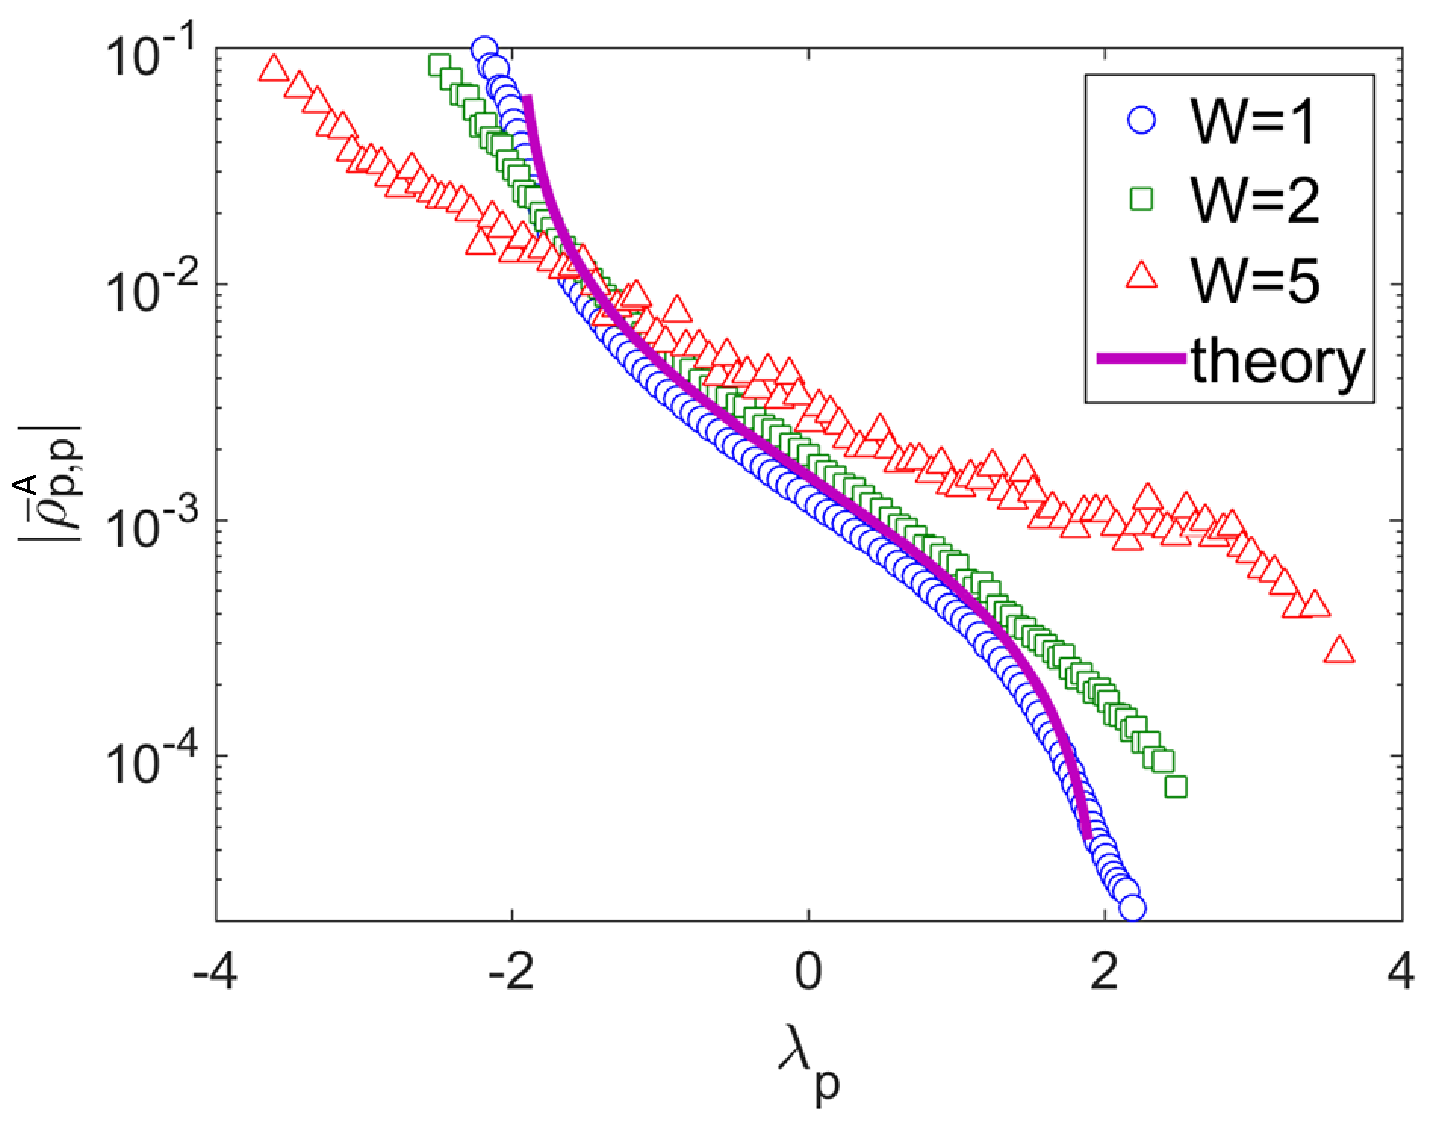
\includegraphics[scale=0.6]{anderson_rho_nn_1}
	}
	\caption{
		Символы "--- усреднённые абсолютные значения диагональных элементов асимптотической матрицы плотности в базисе собственных состояний модели Андерсона как функции усреднённых собственных чисел для синфазной диссипации на соседних сайтах решётки (\(\alpha=0\) и \(l=1\) в уравнении \cref{eq:anderson_diss_local}) для разных значений беспорядка \(W\). Теоретический результат (формула \cref{eq:anderson_diag_mod_8}) показан фиолетовой сплошной линией.
	}
	\label{fig:anderson_rho_nn_1}
\end{figure}

Случай антифазной диссипации на соседних сайтах решетки (\(\alpha=\pi\) и \(l=1\) в уравнении \cref{eq:anderson_diss_local}), из-за симметрии, приводит к обратному выражению для формулы \cref{eq:anderson_diag_mod_8}:
\begin{equation}
\label{eq:anderson_diag_mod_9}
\begin{gathered}
\bar{\rho}^A_{p,p} \approx \frac{2+\lambda_p}{2-\lambda_p}.
\end{gathered}
\end{equation}
Асимптотическая матрица плотности является локализованной возле верхней границы спектра. 
Если фазу диссипации взять равной \(\alpha=\frac{\pi}{2}\), то все диссипативные операторы \cref{eq:anderson_diss_local} окажутся эрмитовыми, что приведёт в итоге систему в тривиальное состояние с максимальной энтропией: \(\rho^A = \frac{\idmtx}{N}\).
При промежуточных значениях фазы диссипации \(0 < \alpha < \frac{\pi}{2}\) (\(\frac{\pi}{2} < \alpha < \pi\)) в асимптотической матрице плотности в базисе собственных состояний модели Андерсона будут преобладать диагональные элементы, локализованные вблизи нижней (верхней) границы спектра собственных значений.

Качественно иная картина наблюдается для диссипативных операторов с \(\alpha=\pi\) и \(l=2\).
В этом случае асимптотическая матрица плотности в исходном базисе \(\rho^A\) является относительно более делокализованной (рисунок~\cref{fig:anderson_rho_loc-3}). 
В то же время, в базисе собственных состояний модели Андерсона \(\bar{\rho}^A\) \cref{eq:anderson_rho_in_eigen_basis} остаётся локализованной со смещением в центр спектра (рисунок~\cref{fig:anderson_rho_loc-4}).
\begin{figure}[ht]
	\centerfloat{
		\hfill
		\subcaptionbox[List-of-Figures entry]{\label{fig:anderson_rho_loc-3}}{%
			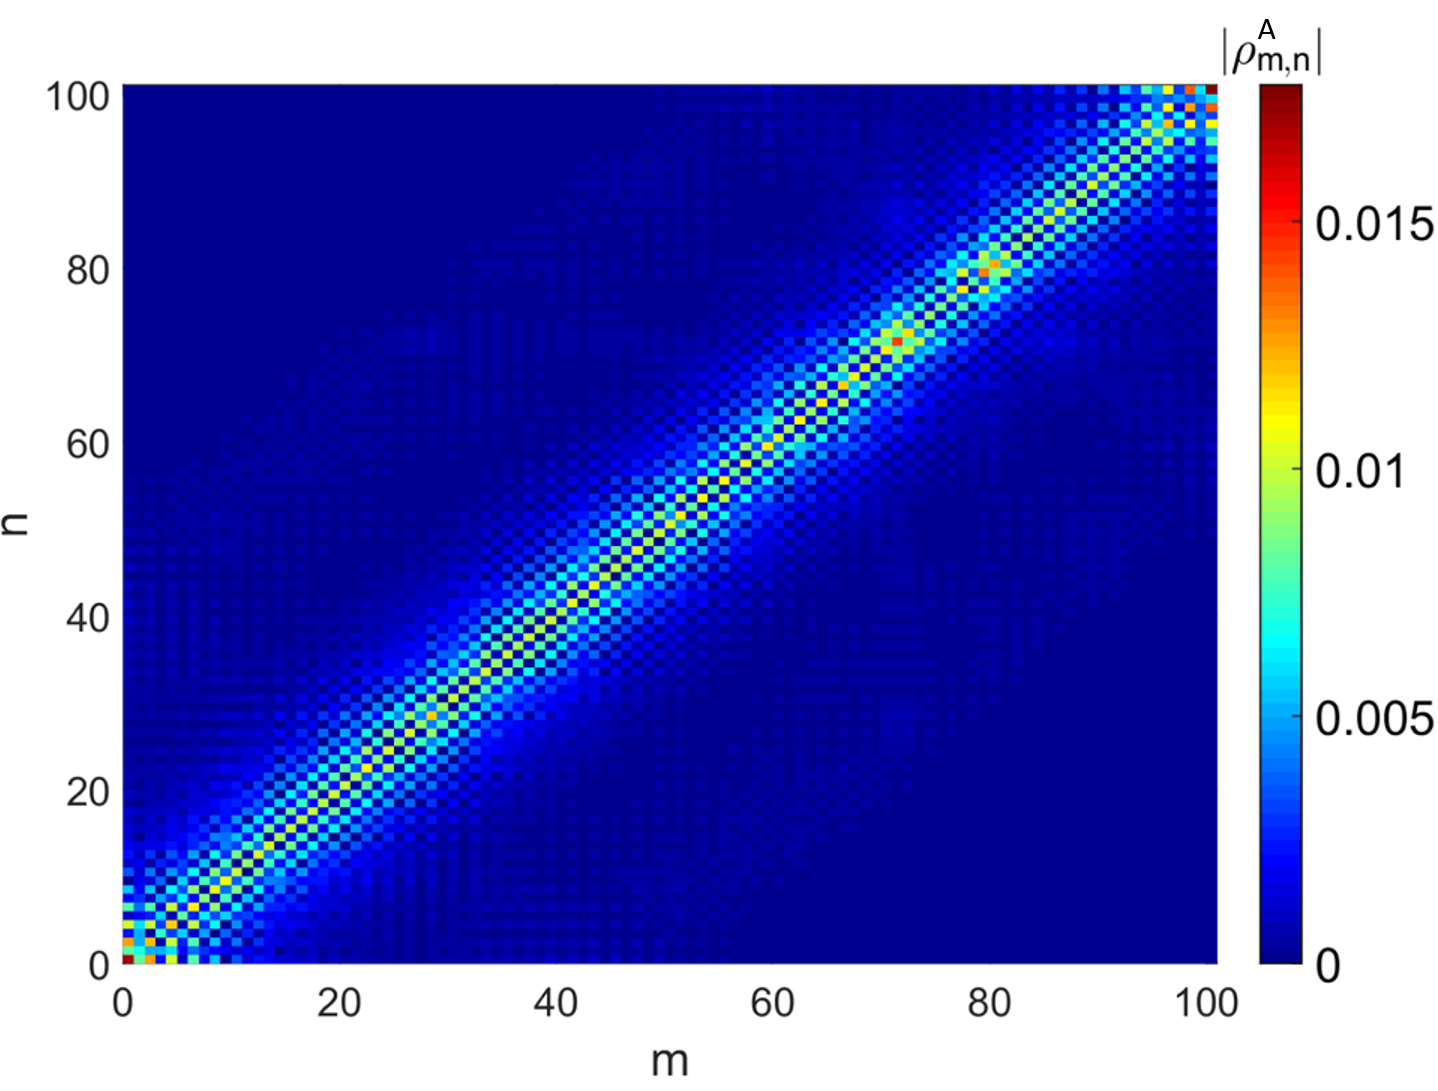
\includegraphics[width=0.5\linewidth]{anderson_rho_loc_3}}
		\hfill
		\subcaptionbox{\label{fig:anderson_rho_loc-4}}{%
			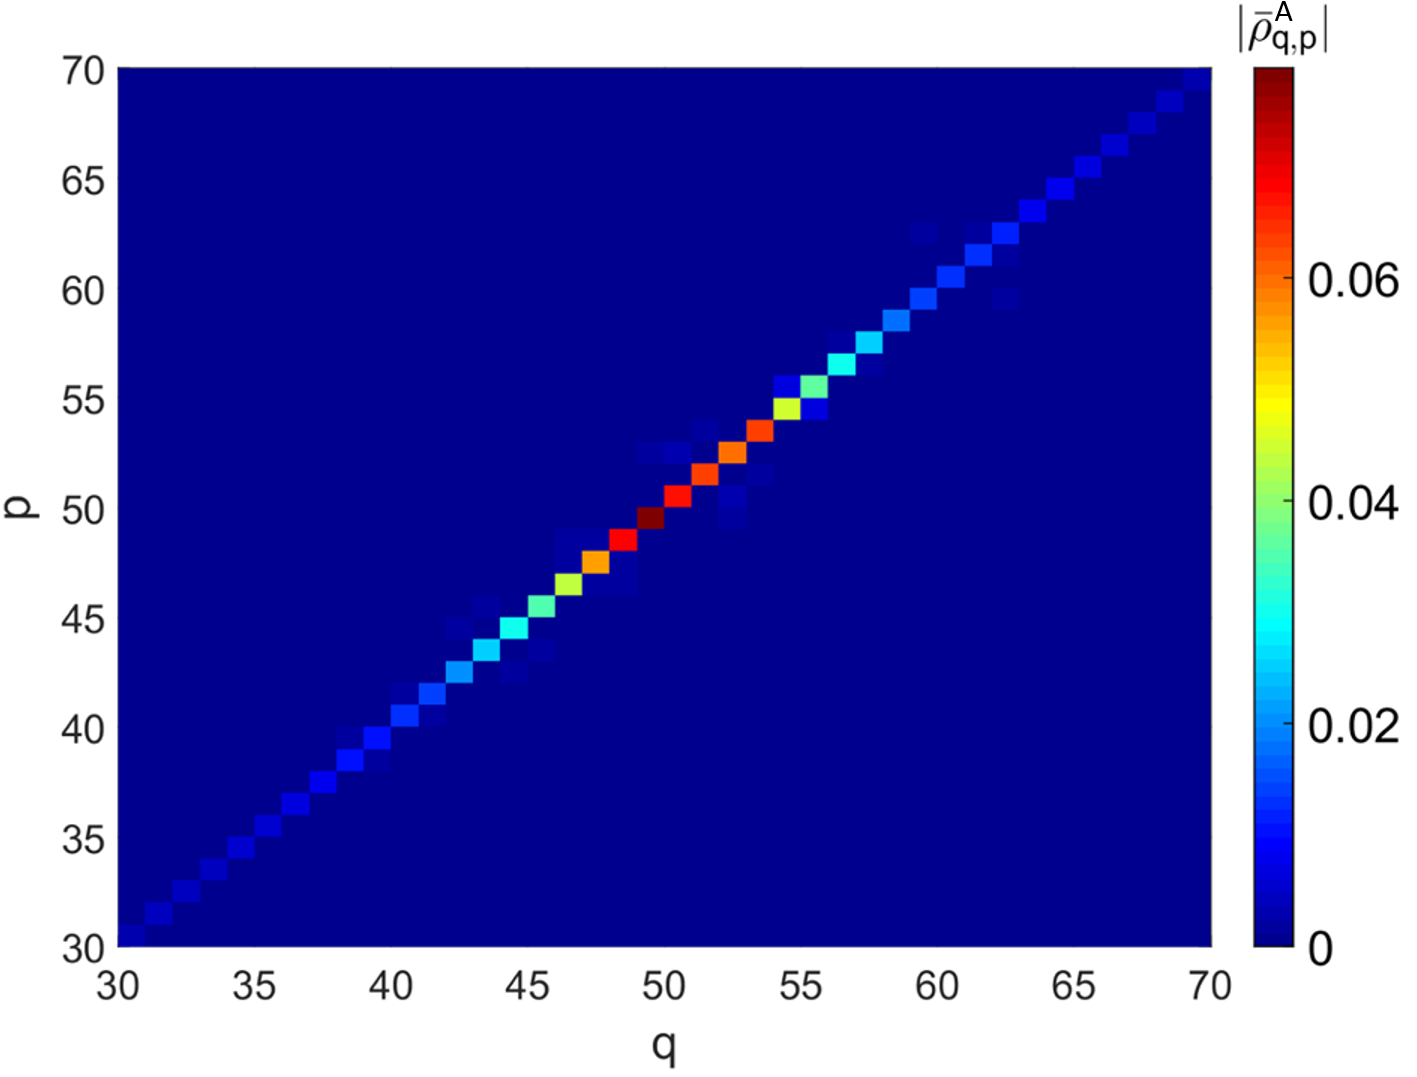
\includegraphics[width=0.5\linewidth]{anderson_rho_loc_4}}
		\hfill
	}
	\legend{}
	\caption[Этот текст попадает в названия рисунков в списке рисунков]
	{
		Абсолютные значения асимптотической матрицы плотности \(\rho^A\) в исходном базисе (a) и в базисе собственных состояний модели Андерсона (б) для единичной реализации беспорядка. Использовались неэрмитовые диссипаторы \cref{eq:anderson_diss_local} c параметрами \(\alpha=\pi\) и \(l=2\). Сила пространственного беспорядка \(W=1\).
	}
	\label{fig:anderson_rho_loc_mid}
\end{figure}
Относительная делокализация в исходном базисе вызвана существенным вкладом собственных состояний из центра спектра, которые имеют относительно большую длину локализации \cref{eq:anderson_loc_length}.
Аналитические соотношения для данного случая выглядят следующим образом:
\begin{equation}
\label{eq:anderson_diag_mod_10}
\begin{gathered}
I^{-}_p = \sum_{k} \left( \mathcal{A}_{p, k+2} \pm \mathcal{A}_{p, k} \right)^2 = \\
= \lambda^2 - 2 \lambda_p \sum_{k} \varepsilon_k \mathcal{A}_{p, k} \mathcal{A}_{p, k+1} + \sum_{k} \varepsilon^2_k \mathcal{A}^2_{p, k} \approx \lambda^2_p + \frac{W^2}{12}, \\
I^{+}_p = 4 - I^{-}_p,
\end{gathered}
\end{equation}
которые в итоге приводят к следующему выражению для диагональных элементов матрицы плотности в базисе собственных состояний модели Андерсона:
\begin{equation}
\label{eq:anderson_diag_mod_11}
\begin{gathered}
\bar{\rho}^A_{p,p} \approx \frac{4}{\lambda^2_p + \frac{W^2}{12}} - 1.
\end{gathered}
\end{equation}
Данное выражение указывает на то, что наибольший вклад в решение вносят собственные состояния из центра спектра.
На рисунке \cref{fig:anderson_rho_nn_2} изображены усреднённые по \(M=100\) случайным реализациям беспорядка диагональные элементы матрицы плотности в базисе собственных состояний модели Андерсона для разных значений силы беспорядка вместе с аналитическим результатом \cref {eq:anderson_diag_mod_11} (сплошные линии). На графике видно хорошее соответствие между численными и аналитическими результатами при малом беспорядке \(W\). При увеличении \(W\) несоответствие увеличивается на краях спектра \(\lambda_p\) ввиду сделанных теоретических приближений. 
\begin{figure}[ht]
	\centerfloat{
		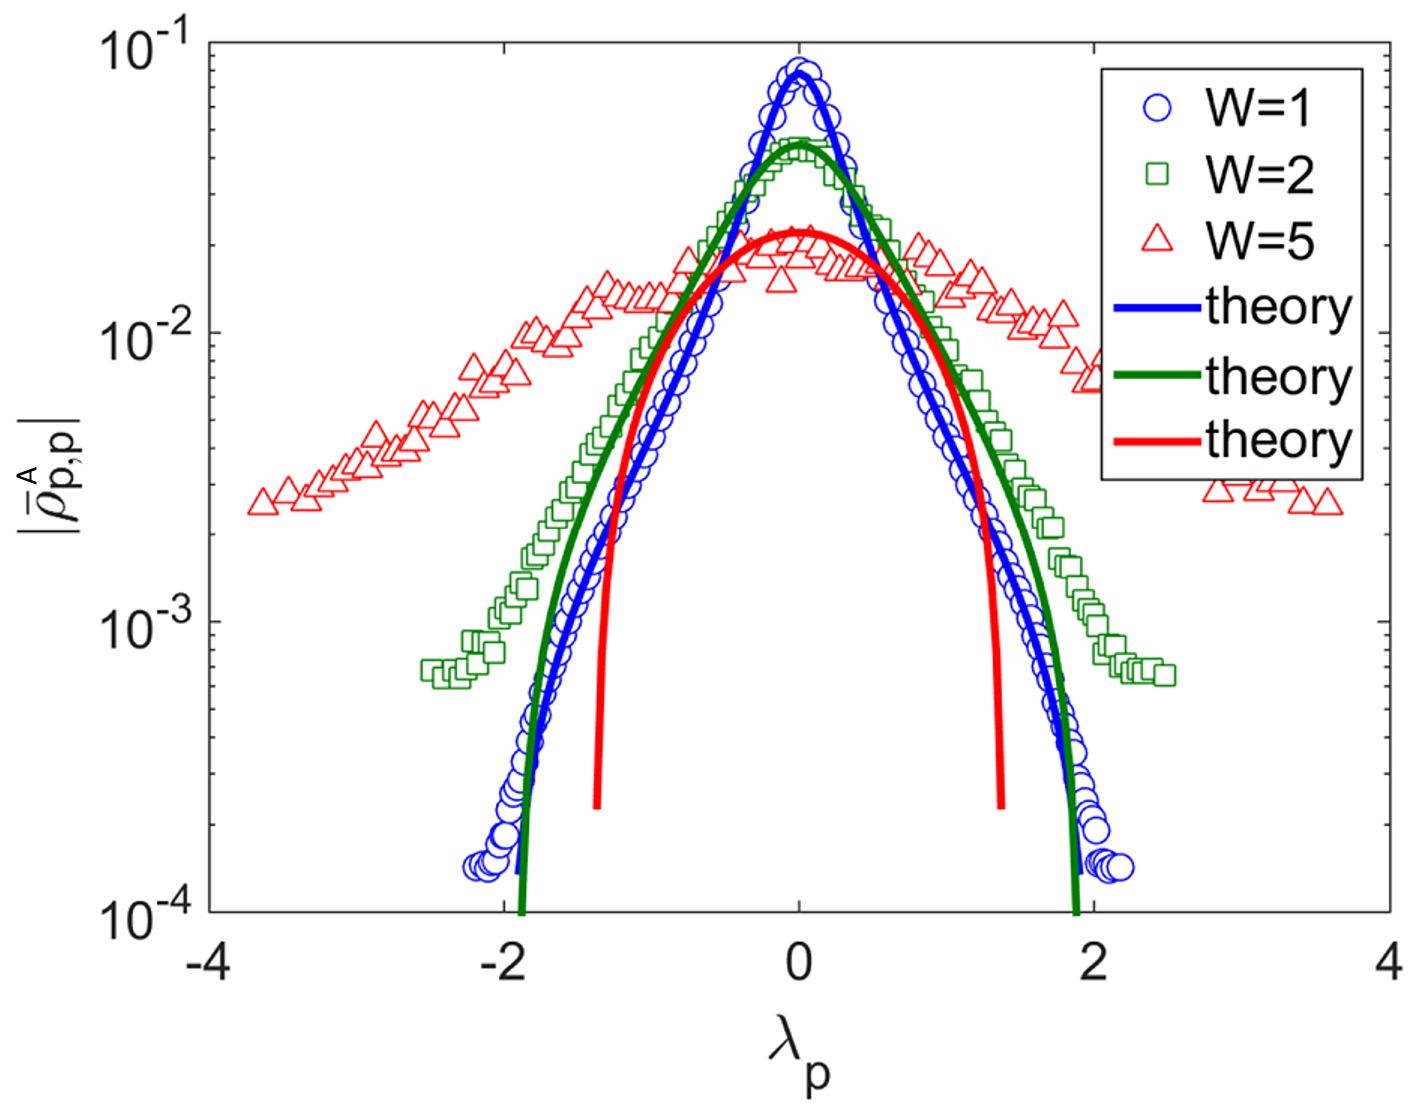
\includegraphics[scale=0.4]{anderson_rho_nn_2}
	}
	\caption{
		Символы "--- усреднённые абсолютные значения диагональных элементов асимптотической матрицы плотности в базисе собственных состояний модели Андерсона как функции усреднённых собственных чисел для синфазной диссипации на соседних сайтах решётки (\(\alpha=\pi\) и \(l=1\) в уравнении \cref{eq:anderson_diss_local}) для разных значений беспорядка \(W\). Теоретический результат (формула \cref{eq:anderson_diag_mod_11}) для каждого значения \(W\) показан соответствующей сплошной линией.
	}
	\label{fig:anderson_rho_nn_2}
\end{figure}

Рассмотрим открытую модель Андерсона \cref{eq:GKSL_lindbladian, eq:anderson_H, eq:anderson_diss_local} c микроскопической точки зрения, используя метод квантовых тректорий, описанный в разделе \cref{sec:ch1/sec2}. Квантовая траектория с индексом \(j\) будет описываться волновой функцией \(\left| \psi_j(t) \right\rangle\). Зафиксируем случайный беспорядок  силой \(W=1\) в системе и время переходного процесса \(t^A = 10^4\) "--- достаточным до достижения каждой траектории аттрактора (асимптотической матрицы плотности \(\rho^A\)). После достижения аттрактора за каждой квантовой траекторией будет вестись наблюдение в течении \(t^F = 10^4\) (суммарное время пропагации \(t = t^A + t^F\)). Количество рассматриваемых квантовых траекторий \(M_r=10^6\). Для каждой \(j\)-ой квантовой траектории будут рассматриваться позиция и энергия, вычисляемые по соответствующим формулам:
\begin{equation}
\label{eq:anderson_position}
\begin{gathered}
n_j(t) = \langle \psi_j(t)| O_n | \psi_j(t) \rangle,
\end{gathered}
\end{equation}
\begin{equation}
\label{eq:anderson_energy}
\begin{gathered}
E_j(t) = \langle \psi_j(t)| H | \psi_j(t) \rangle,
\end{gathered}
\end{equation}
где \(O_n\) - матрица оператора числа частиц, а \(H\) - гамильтониан модели Андерсона \cref{eq:anderson_H}.

\begin{figure}[ht]
	\centerfloat{
		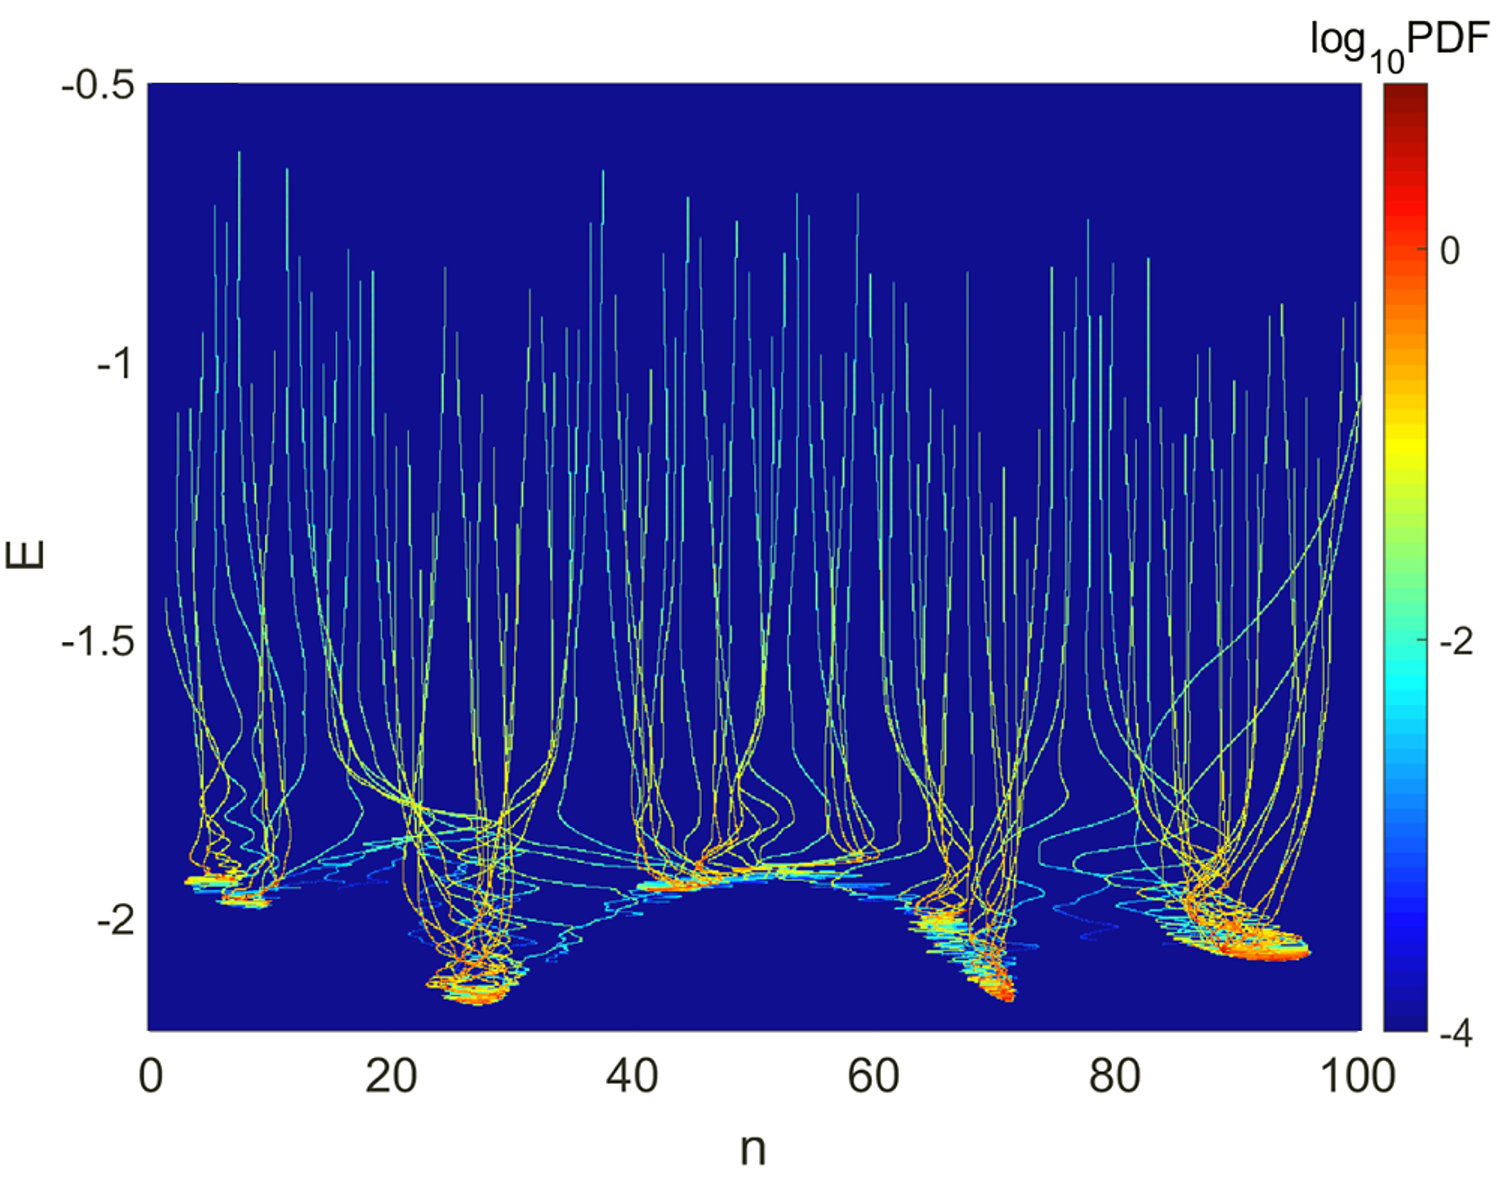
\includegraphics[scale=0.4]{anderson_qj_1}
	}
	\caption{
		Функция распределения плотности вероятностей (PDF) квантовых траекторий на плоскости позиции \(n(t)\) и энергии \(E(t))\) для случая синфазной диссипации на соседних сайтах решётки (\(\alpha=0\) и \(l=1\) в \cref{eq:anderson_diss_local}).
	}
	\label{fig:anderson_qj_1}
\end{figure}

На рисунке \cref{fig:anderson_qj_1} изображена двумерная функция распределения плотности вероятностей (probability densidy function - PDF) на плоскости позиции \(n(t)\) \cref{eq:anderson_position} и энергии \(E(t))\) , построенная для \(M_r=10^6\) траекторий, наблюдаемых в течение \(t^F=10^4\) времени для случая синфазной диссипации на соседних сайтах решётки (\(\alpha=0\) и \(l=1\) в \cref{eq:anderson_diss_local}). Динамика отдельных квантовых траекторий представляет собой длительные «залипания» вблизи центров локализации (красные области на рисунке \cref{fig:anderson_qj_1}), вызванные эволюцией с неэрмитовым гамильтонианом \cref{eq:H_nonhermit} (алгоритм \ref{alg:qt_main}). Данные процессы прерываются квантовыми скачками (алгоритм \ref{alg:qt_jump}), которые накачивают систему энергией и переносят траектории в бледно-голубые «истоки» в верхней части рисунка \cref{fig:anderson_qj_1}, откуда системы быстро релаксирует по структурированной сети к одному из собственных состояний модели Андерсона. Структура сети не меняется при дальнейшем увеличении числа траекторий \(M_r\).

Результаты \cite{Yusipov2017}, представленные в данном разделе, указывают на то, что в открытых квантовых системах с физически реализуемой диссипацией возможно создание стационарных состояний, которые доминируют несколько локализованных мод пространственно неоднородного гамильтониана из классической модели Андерсона. Андерсоновские моды выбираются в соответствии с их пространственно-фазовыми свойствами, унаследованными от собственных состояний гамильтониана в пределе нулевого беспорядка \cite{Ishii1973}, с использованием фазо-параметризованных диссипативных операторов. Изменение фазы диссипативных операторов изменяет локализационные свойства системы.
 
\section{Управление одночастичной локализацией в открытых квантовых системах}\label{sec:ch1/epjb}
В данном разделе будет изучено влияние параметров диссипативных операторов \cref{eq:anderson_diss_local} на локализационные свойства открытой квантовой системы \cref{eq:GKSL_lindbladian,eq:anderson_H}, а также влияние добавочной дефазирующей диссипации \cref{eq:anderson_diss_dephase} на асимптотическое состояние системы.

Рассмотрим случай синфазной диссипации на соседних сайтах решётки (\(\alpha=0\) и \(l=1\) в \cref{eq:anderson_diss_local} с коэффициентами скорости диссипации \(\gamma^l = 0.1\). Добавим к данной модели дополнительные дефазирующие \cref{eq:anderson_diss_dephase} каналы рассеивания с коэффициентами скорости \(\gamma^d\). На рисунке \cref{fig:anderson_rho_nn_with_dephasing} изображены диагональные элементы асимптотической матрицы плотности в базисе собственных состояний модели Андерсона со смешанным типом диссипации для разных значений \(\gamma^d\). Стоить отметить, что не только слабая \(\gamma^d \ll \gamma^l\), но и сильная \(\gamma^d \gg \gamma^l\) дефазирующая диссипация не уничтожает спектральную диссипацию и структурно не изменяет решение (преобладают собственные состояния из той же части спектра).

\begin{figure}[ht]
	\centerfloat{
		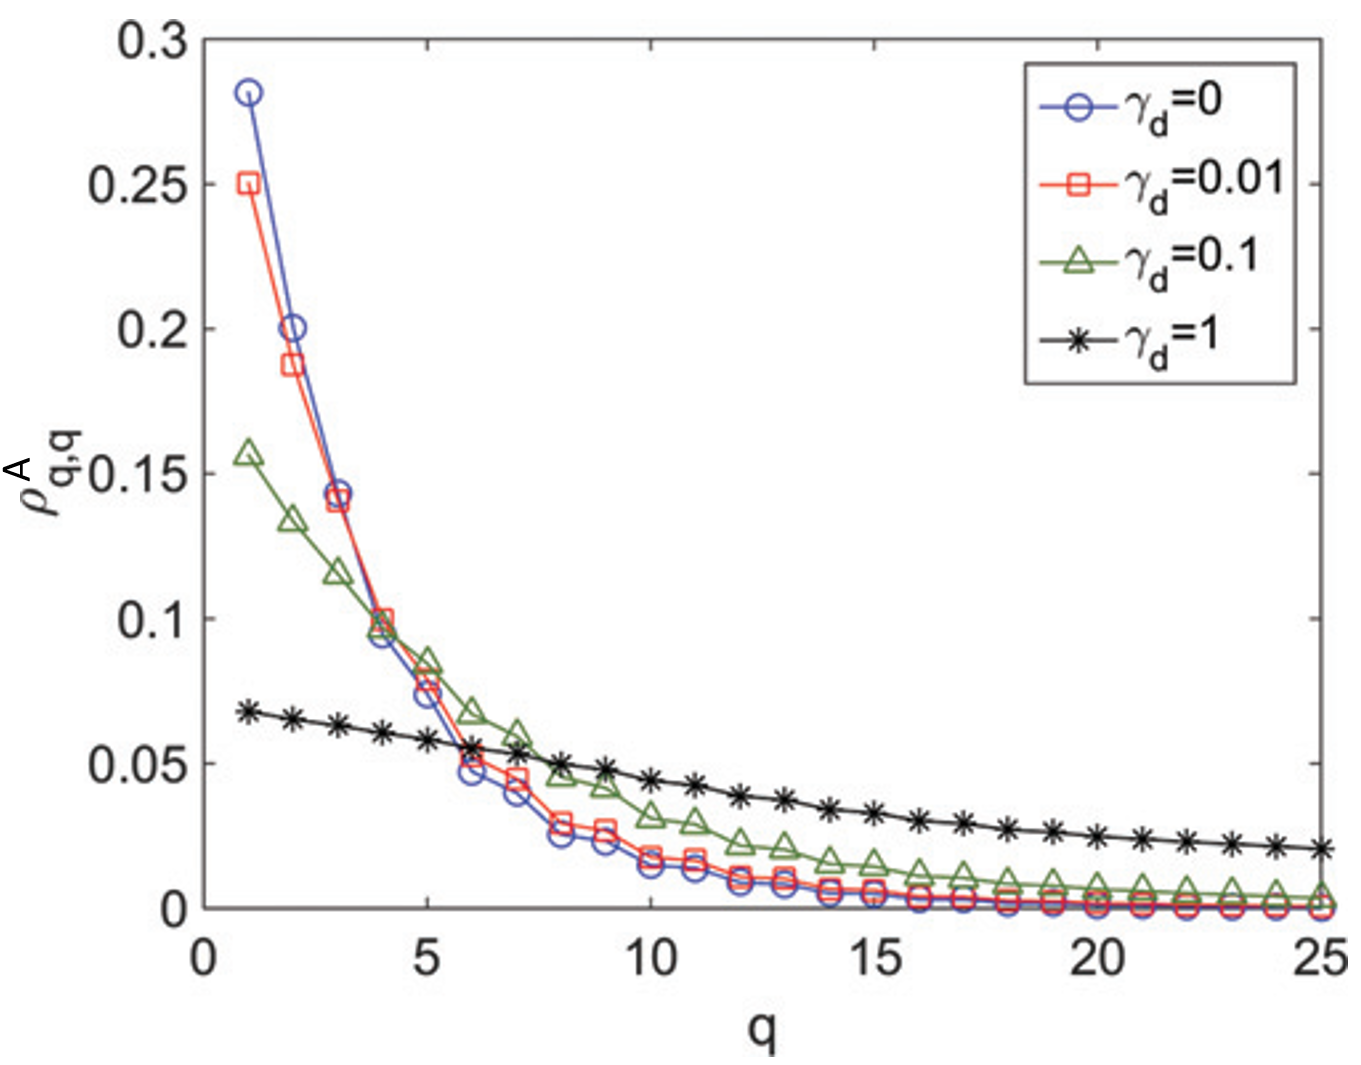
\includegraphics[scale=0.4]{anderson_rho_nn_with_dephasing}
	}
	\caption{
		Диагональные элементы асимптотической матрицы плотности в базисе собственных состояний модели Андерсона \(\rho^A\) для случая синфазной диссипации на соседних сайтах решётки (\(\alpha=0\) и \(l=1\) в \cref{eq:anderson_diss_local} и скорость диссипации \(\gamma^l=0.1\)) в комбинации с дефазирующей диссипацией (\cref{eq:anderson_diss_dephase} и скорость диссипации \(\gamma^d\)) для разных значений \(\gamma^d\). Размер системы \(N=25\), сила пространственного беспорядка \(W=2\). Усреднение производилось для \(N_r = 10^3\) реализаций беспорядка. 
	}
	\label{fig:anderson_rho_nn_with_dephasing}
\end{figure}

Рассмотрим теперь систему в пределе нулевого беспорядка. Базис системы состоит из плоских волн с соответсвующим спектром собственных значений:
\begin{equation}
\label{eq:anderson_plane_wave}
\begin{gathered}
\phi_j = \frac{e^{i j k}}{\sqrt{N}}, \\
\lambda_k = -2 \cos{k}, \\
k = \frac{2 \pi q}{N}, \\
q = -\frac{N}{2}, \ldots, \frac{N}{2}.
\end{gathered}
\end{equation}
Можно заметить, что для конкретного значения фазы диссипатора \cref{eq:anderson_diss_local} \(\alpha = \frac{2 \pi q}{N}\), плоская  \cref{eq:anderson_plane_wave} с соответствующим \(k=\alpha\) является «тёмным» состоянием для всех диссипативных операторов \cref{eq:anderson_diss_local} \cite{Diehl2008, Kraus2008}, в то время как все остальные собственные состояния не являются.
В этом случае (когда нет дефазирующей добавки \(\gamma^d = 0\)), плоская волна с \(k = \alpha\) является асимптотическим состоянием открытой квантовой системы. 
В том случае, когда \(\alpha\) не совпадает точно со значением \(k\) или присутствует дефазирующая диссипация, асимптотическое состояние остаётся очень близким к исходному «тёмному» состоянию, причём наибольший вклад вносят плоские волны с \(k \approx \alpha\) (рисунок \cref{fig:anderson_rho_nn_zero_disorder}).
\begin{figure}[ht]
	\centerfloat{
		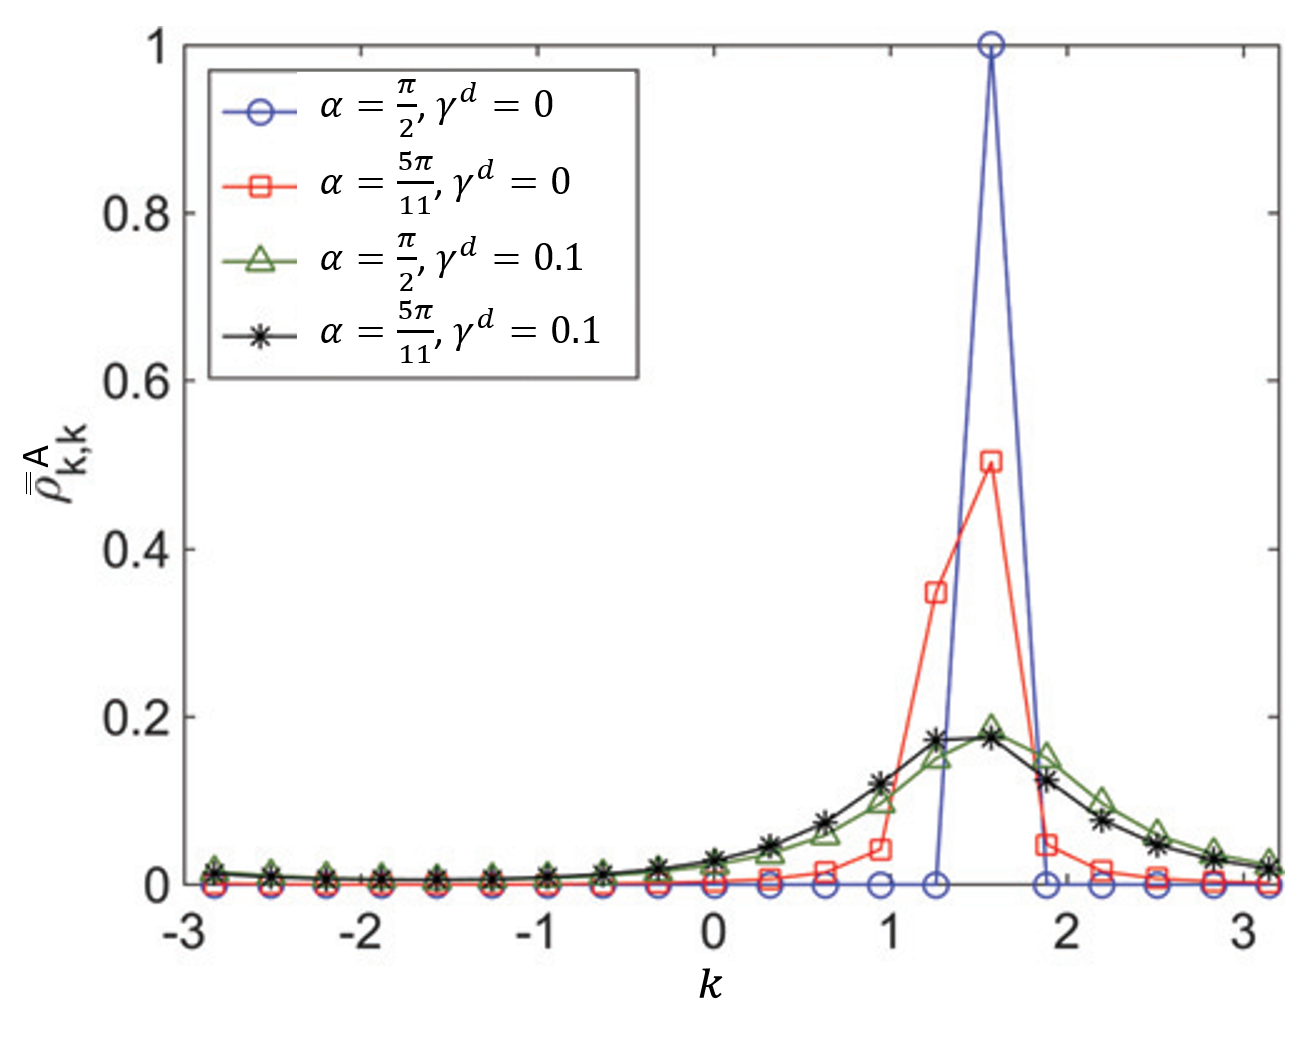
\includegraphics[scale=0.4]{anderson_rho_nn_zero_disorder}
	}
	\caption{
		Диагональные элементы асимптотической матрицы плотности в базисе плоских волн \cref{eq:anderson_plane_wave} для случая синфазной диссипации на соседних сайтах решётки (\(\alpha=0\) и \(l=1\) в \cref{eq:anderson_diss_local} и скорость диссипации \(\gamma^l=0.1\)) в комбинации с дефазирующей диссипацией (\cref{eq:anderson_diss_dephase} и скорость диссипации \(\gamma^d\)). Размер системы \(N=20\), сила пространственного беспорядка \(W=0\).
	}
	\label{fig:anderson_rho_nn_zero_disorder}
\end{figure}





Мы можем сделать \textbf{жирный текст} и \textit{курсив}.


Сошлёмся на библиографию.
Одна ссылка: \cite[с.~54]{Sokolov}\cite[с.~36]{Methodology}.
Две ссылки: \cite{Sokolov,Gaidaenko}.
Ссылка на собственные работы: \cite{Sokolov, Gaidaenko}.
Много ссылок: %\cite[с.~54]{Lermontov,Management,Borozda} % такой «фокус»
%вызывает biblatex warning относительно опции sortcites, потому что неясно, к
%какому источнику относится уточнение о страницах, а bibtex об этой проблеме
%даже не предупреждает
\cite{Lermontov, Management, Borozda, Marketing, Constitution, FamilyCode,
	Gost.7.0.53, Razumovski, Lagkueva, Pokrovski, Methodology, Berestova,
	Kriger}%
\ifnumequal{\value{bibliosel}}{0}{% Примеры для bibtex8
	\cite{Sirotko, Lukina, Encyclopedia, Nasirova}%
}{% Примеры для biblatex через движок biber
	\cite{Sirotko2, Lukina2, Encyclopedia2, Nasirova2}%
}%
.
И~ещё немного ссылок:~\cite{Article,Book,Booklet,Conference,Inbook,Incollection,Manual,Mastersthesis,
	Misc,Phdthesis,Proceedings,Techreport,Unpublished}
% Следует обратить внимание, что пробел после запятой внутри \cite{}
% обрабатывается ожидаемо, а пробел перед запятой, может вызывать проблемы при
% обработке ссылок.
\cite{medvedev2006jelektronnye, CEAT:CEAT581, doi:10.1080/01932691.2010.513279,
	Gosele1999161,Li2007StressAnalysis, Shoji199895, test:eisner-sample,
	test:eisner-sample-shorted, AB_patent_Pomerantz_1968, iofis_patent1960}
\ifnumequal{\value{bibliosel}}{0}{% Примеры для bibtex8
}{% Примеры для biblatex через движок biber
	\cite{patent2h, patent3h, patent2}%
}%
.

\ifnumequal{\value{bibliosel}}{0}{% Примеры для bibtex8
	Попытка реализовать несколько ссылок на конкретные страницы
	для \texttt{bibtex} реализации библиографии:
	[\citenum{Sokolov}, с.~54; \citenum{Gaidaenko}, с.~36].
}{% Примеры для biblatex через движок biber
	Несколько источников (мультицитата):
	% Тут специально написано по-разному тире, для демонстрации, что
	% применение специальных тире в настоящий момент в biblatex приводит к непоказу
	% "с.".
	\cites[vii--x, 5, 7]{Sokolov}[v"--~x, 25, 526]{Gaidaenko}[vii--x, 5, 7]{Techreport},
	работает только в \texttt{biblatex} реализации библиографии.
}%

Ссылки на собственные работы:~\cite{Sokolov, Gaidaenko}

Сошлёмся на приложения: Приложение~\cref{app:A}, Приложение~\cref{app:B2}.

Сошлёмся на формулу: формула~\cref{eq:equation1}.

Сошлёмся на изображение: рисунок~\cref{fig:knuth}.

Стандартной практикой является добавление к ссылкам префикса, характеризующего тип элемента.
Это не является строгим требованием, но~позволяет лучше ориентироваться в документах большого размера.
Например, для ссылок на~рисунки используется префикс \textit{fig},
для ссылки на~таблицу "--- \textit{tab}.

В таблице \cref{tab:tab_pref} приложения~\cref{app:B4} приведён список рекомендуемых
к использованию стандартных префиксов.

Благодаря пакету \textit{icomma}, \LaTeX~одинаково хорошо воспринимает
в~качестве десятичного разделителя и запятую (\(3,1415\)), и точку (\(3.1415\)).

\subsection{Ненумерованные одиночные формулы}\label{subsec:ch1/sec3/sub1}

Вот так может выглядеть формула, которую необходимо вставить в~строку
по~тексту: \(x \approx \sin x\) при \(x \to 0\).

А вот так выглядит ненумерованная отдельностоящая формула c подстрочными
и надстрочными индексами:
\[
(x_1+x_2)^2 = x_1^2 + 2 x_1 x_2 + x_2^2
\]

Формула с неопределенным интегралом:
\[
\int f(\alpha+x)=\sum\beta
\]

При использовании дробей формулы могут получаться очень высокие:
\[
  \frac{1}{\sqrt{2}+
  \displaystyle\frac{1}{\sqrt{2}+
  \displaystyle\frac{1}{\sqrt{2}+\cdots}}}
\]

В формулах можно использовать греческие буквы:
%Все \original... команды заранее, ради этого примера, определены в Dissertation\userstyles.tex
\[
\alpha\beta\gamma\delta\originalepsilon\epsilon\zeta\eta\theta%
\vartheta\iota\kappa\varkappa\lambda\mu\nu\xi\pi\varpi\rho\varrho%
\sigma\varsigma\tau\upsilon\originalphi\phi\chi\psi\omega\Gamma\Delta%
\Theta\Lambda\Xi\Pi\Sigma\Upsilon\Phi\Psi\Omega
\]
\[%https://texfaq.org/FAQ-boldgreek
\boldsymbol{\alpha\beta\gamma\delta\originalepsilon\epsilon\zeta\eta%
\theta\vartheta\iota\kappa\varkappa\lambda\mu\nu\xi\pi\varpi\rho%
\varrho\sigma\varsigma\tau\upsilon\originalphi\phi\chi\psi\omega\Gamma%
\Delta\Theta\Lambda\Xi\Pi\Sigma\Upsilon\Phi\Psi\Omega}
\]

Для добавления формул можно использовать пары \verb+$+\dots\verb+$+ и \verb+$$+\dots\verb+$$+,
но~они считаются устаревшими.
Лучше использовать их функциональные аналоги \verb+\(+\dots\verb+\)+ и \verb+\[+\dots\verb+\]+.

\subsection{Ненумерованные многострочные формулы}\label{subsec:ch1/sec3/sub2}

Вот так можно написать две формулы, не нумеруя их, чтобы знаки <<равно>> были
строго друг под другом:
\begin{align}
  f_W & =  \min \left( 1, \max \left( 0, \frac{W_{soil} / W_{max}}{W_{crit}} \right)  \right), \nonumber \\
  f_T & =  \min \left( 1, \max \left( 0, \frac{T_s / T_{melt}}{T_{crit}} \right)  \right), \nonumber
\end{align}

Выровнять систему ещё и по переменной \( x \) можно, используя окружение
\verb|alignedat| из пакета \verb|amsmath|. Вот так:
\[
    |x| = \left\{
    \begin{alignedat}{2}
        &&x, \quad &\text{eсли } x\geqslant 0 \\
        &-&x, \quad & \text{eсли } x<0
    \end{alignedat}
    \right.
\]
Здесь первый амперсанд (в исходном \LaTeX\ описании формулы) означает
выравнивание по~левому краю, второй "--- по~\( x \), а~третий "--- по~слову
<<если>>. Команда \verb|\quad| делает большой горизонтальный пробел.

Ещё вариант:
\[
    |x|=
    \begin{cases}
    \phantom{-}x, \text{если } x \geqslant 0 \\
    -x, \text{если } x<0
    \end{cases}
\]

Кроме того, для  нумерованных формул \verb|alignedat| делает вертикальное
выравнивание номера формулы по центру формулы. Например, выравнивание
компонент вектора:
\begin{equation}
\label{eq:2p3}
\begin{alignedat}{2}
{\mathbf{N}}_{o1n}^{(j)} = \,{\sin} \phi\,n\!\left(n+1\right)
         {\sin}\theta\,
         \pi_n\!\left({\cos} \theta\right)
         \frac{
               z_n^{(j)}\!\left( \rho \right)
              }{\rho}\,
           &{\boldsymbol{\hat{\mathrm e}}}_{r}\,+   \\
+\,
{\sin} \phi\,
         \tau_n\!\left({\cos} \theta\right)
         \frac{
            \left[\rho z_n^{(j)}\!\left( \rho \right)\right]^{\prime}
              }{\rho}\,
            &{\boldsymbol{\hat{\mathrm e}}}_{\theta}\,+   \\
+\,
{\cos} \phi\,
         \pi_n\!\left({\cos} \theta\right)
         \frac{
            \left[\rho z_n^{(j)}\!\left( \rho \right)\right]^{\prime}
              }{\rho}\,
            &{\boldsymbol{\hat{\mathrm e}}}_{\phi}\:.
\end{alignedat}
\end{equation}

Ещё об отступах. Иногда для лучшей <<читаемости>> формул полезно
немного исправить стандартные интервалы \LaTeX\ с учётом логической
структуры самой формулы. Например в формуле~\cref{eq:2p3} добавлен
небольшой отступ \verb+\,+ между основными сомножителями, ниже
результат применения всех вариантов отступа:
\begin{align*}
\backslash! &\quad f(x) = x^2\! +3x\! +2 \\
  \mbox{по-умолчанию} &\quad f(x) = x^2+3x+2 \\
\backslash, &\quad f(x) = x^2\, +3x\, +2 \\
\backslash{:} &\quad f(x) = x^2\: +3x\: +2 \\
\backslash; &\quad f(x) = x^2\; +3x\; +2 \\
\backslash \mbox{space} &\quad f(x) = x^2\ +3x\ +2 \\
\backslash \mbox{quad} &\quad f(x) = x^2\quad +3x\quad +2 \\
\backslash \mbox{qquad} &\quad f(x) = x^2\qquad +3x\qquad +2
\end{align*}

Можно использовать разные математические алфавиты:
\begin{align}
\mathcal{ABCDEFGHIJKLMNOPQRSTUVWXYZ} \nonumber \\
\mathfrak{ABCDEFGHIJKLMNOPQRSTUVWXYZ} \nonumber \\
\mathbb{ABCDEFGHIJKLMNOPQRSTUVWXYZ} \nonumber
\end{align}

Посмотрим на систему уравнений на примере аттрактора Лоренца:

\[
\left\{
  \begin{array}{rl}
    \dot x = & \sigma (y-x) \\
    \dot y = & x (r - z) - y \\
    \dot z = & xy - bz
  \end{array}
\right.
\]

А для вёрстки матриц удобно использовать многоточия:
\[
\left(
  \begin{array}{ccc}
    a_{11} & \ldots & a_{1n} \\
    \vdots & \ddots & \vdots \\
    a_{n1} & \ldots & a_{nn} \\
  \end{array}
\right)
\]

\subsection{Нумерованные формулы}\label{subsec:ch1/sec3/sub3}

А вот так пишется нумерованная формула:
\begin{equation}
  \label{eq:equation1}
  e = \lim_{n \to \infty} \left( 1+\frac{1}{n} \right) ^n
\end{equation}

Нумерованных формул может быть несколько:
\begin{equation}
  \label{eq:equation2}
  \lim_{n \to \infty} \sum_{k=1}^n \frac{1}{k^2} = \frac{\pi^2}{6}
\end{equation}

Впоследствии на формулы~\cref{eq:equation1, eq:equation2} можно ссылаться.

Сделать так, чтобы номер формулы стоял напротив средней строки, можно,
используя окружение \verb|multlined| (пакет \verb|mathtools|) вместо
\verb|multline| внутри окружения \verb|equation|. Вот так:
\begin{equation} % \tag{S} % tag - вписывает свой текст
  \label{eq:equation3}
    \begin{multlined}
        1+ 2+3+4+5+6+7+\dots + \\
        + 50+51+52+53+54+55+56+57 + \dots + \\
        + 96+97+98+99+100=5050
    \end{multlined}
\end{equation}

Уравнения~\cref{eq:subeq_1,eq:subeq_2} демонстрируют возможности
окружения \verb|\subequations|.
\begin{subequations}
    \label{eq:subeq_1}
    \begin{gather}
        y = x^2 + 1 \label{eq:subeq_1-1} \\
        y = 2 x^2 - x + 1 \label{eq:subeq_1-2}
    \end{gather}
\end{subequations}
Ссылки на отдельные уравнения~\cref{eq:subeq_1-1,eq:subeq_1-2,eq:subeq_2-1}.
\begin{subequations}
    \label{eq:subeq_2}
    \begin{align}
        y &= x^3 + x^2 + x + 1 \label{eq:subeq_2-1} \\
        y &= x^2
    \end{align}
\end{subequations}

\subsection{Форматирование чисел и размерностей величин}\label{sec:units}

Числа форматируются при помощи команды \verb|\num|:
\num{5,3};
\num{2,3e8};
\num{12345,67890};
\num{2,6 d4};
\num{1+-2i};
\num{.3e45};
\num[exponent-base=2]{5 e64};
\num[exponent-base=2,exponent-to-prefix]{5 e64};
\num{1.654 x 2.34 x 3.430}
\num{1 2 x 3 / 4}.
Для написания последовательности чисел можно использовать команды \verb|\numlist| и \verb|\numrange|:
\numlist{10;30;50;70}; \numrange{10}{30}.
Значения углов можно форматировать при помощи команды \verb|\ang|:
\ang{2.67};
\ang{30,3};
\ang{-1;;};
\ang{;-2;};
\ang{;;-3};
\ang{300;10;1}.

Обратите внимание, что ГОСТ запрещает использование знака <<->> для обозначения отрицательных чисел
за исключением формул, таблиц и~рисунков.
Вместо него следует использовать слово <<минус>>.

Размерности можно записывать при помощи команд \verb|\si| и \verb|\SI|:
\si{\farad\squared\lumen\candela};
\si{\joule\per\mole\per\kelvin};
\si[per-mode = symbol-or-fraction]{\joule\per\mole\per\kelvin};
\si{\metre\per\second\squared};
\SI{0.10(5)}{\neper};
\SI{1.2-3i e5}{\joule\per\mole\per\kelvin};
\SIlist{1;2;3;4}{\tesla};
\SIrange{50}{100}{\volt}.
Список единиц измерений приведён в таблицах~\cref{tab:unit:base,
tab:unit:derived,tab:unit:accepted,tab:unit:physical,tab:unit:other}.
Приставки единиц приведены в~таблице~\cref{tab:unit:prefix}.

С дополнительными опциями форматирования можно ознакомиться в~описании пакета \texttt{siunitx};
изменить или добавить единицы измерений можно в~файле \texttt{siunitx.cfg}.

\begin{table}
    \centering
    \captionsetup{justification=centering} % выравнивание подписи по-центру
    \caption{Основные величины СИ}\label{tab:unit:base}
    \begin{tabular}{llc}
        \toprule
        Название  & Команда                & Символ         \\
        \midrule
        Ампер     & \verb|\ampere| & \si{\ampere}   \\
        Кандела   & \verb|\candela| & \si{\candela}  \\
        Кельвин   & \verb|\kelvin| & \si{\kelvin}   \\
        Килограмм & \verb|\kilogram| & \si{\kilogram} \\
        Метр      & \verb|\metre| & \si{\metre}    \\
        Моль      & \verb|\mole| & \si{\mole}     \\
        Секунда   & \verb|\second| & \si{\second}   \\
        \bottomrule
    \end{tabular}
\end{table}

\begin{table}
  \small
  \centering
  \begin{threeparttable}% выравнивание подписи по границам таблицы
    \caption{Производные единицы СИ}\label{tab:unit:derived}
    \begin{tabular}{llc|llc}
        \toprule
        Название       & Команда                 & Символ              & Название & Команда & Символ \\
        \midrule
        Беккерель      & \verb|\becquerel|  & \si{\becquerel}     &
        Ньютон         & \verb|\newton|  & \si{\newton}                                      \\
        Градус Цельсия & \verb|\degreeCelsius| & \si{\degreeCelsius} &
        Ом             & \verb|\ohm| & \si{\ohm}                                         \\
        Кулон          & \verb|\coulomb| & \si{\coulomb}       &
        Паскаль        & \verb|\pascal| & \si{\pascal}                                      \\
        Фарад          & \verb|\farad| & \si{\farad}         &
        Радиан         & \verb|\radian| & \si{\radian}                                      \\
        Грей           & \verb|\gray| & \si{\gray}          &
        Сименс         & \verb|\siemens| & \si{\siemens}                                     \\
        Герц           & \verb|\hertz| & \si{\hertz}         &
        Зиверт         & \verb|\sievert| & \si{\sievert}                                     \\
        Генри          & \verb|\henry| & \si{\henry}         &
        Стерадиан      & \verb|\steradian| & \si{\steradian}                                   \\
        Джоуль         & \verb|\joule| & \si{\joule}         &
        Тесла          & \verb|\tesla| & \si{\tesla}                                       \\
        Катал          & \verb|\katal| & \si{\katal}         &
        Вольт          & \verb|\volt| & \si{\volt}                                        \\
        Люмен          & \verb|\lumen| & \si{\lumen}         &
        Ватт           & \verb|\watt| & \si{\watt}                                        \\
        Люкс           & \verb|\lux| & \si{\lux}           &
        Вебер          & \verb|\weber| & \si{\weber}                                       \\
        \bottomrule
    \end{tabular}
  \end{threeparttable}
\end{table}

\begin{table}
  \centering
  \begin{threeparttable}% выравнивание подписи по границам таблицы
    \caption{Внесистемные единицы}\label{tab:unit:accepted}

    \begin{tabular}{llc}
        \toprule
        Название        & Команда                 & Символ          \\
        \midrule
        День            & \verb|\day| & \si{\day}       \\
        Градус          & \verb|\degree| & \si{\degree}    \\
        Гектар          & \verb|\hectare| & \si{\hectare}   \\
        Час             & \verb|\hour| & \si{\hour}      \\
        Литр            & \verb|\litre| & \si{\litre}     \\
        Угловая минута  & \verb|\arcminute| & \si{\arcminute} \\
        Угловая секунда & \verb|\arcsecond| & \si{\arcsecond} \\ %
        Минута          & \verb|\minute| & \si{\minute}    \\
        Тонна           & \verb|\tonne| & \si{\tonne}     \\
        \bottomrule
    \end{tabular}
  \end{threeparttable}
\end{table}

\begin{table}
    \centering
    \captionsetup{justification=centering}
    \caption{Внесистемные единицы, получаемые из эксперимента}\label{tab:unit:physical}
    \begin{tabular}{llc}
        \toprule
        Название                & Команда                 & Символ                 \\
        \midrule
        Астрономическая единица & \verb|\astronomicalunit| & \si{\astronomicalunit} \\
        Атомная единица массы   & \verb|\atomicmassunit| & \si{\atomicmassunit}   \\
        Боровский радиус        & \verb|\bohr| & \si{\bohr}             \\
        Скорость света          & \verb|\clight| & \si{\clight}           \\
        Дальтон                 & \verb|\dalton| & \si{\dalton}           \\
        Масса электрона         & \verb|\electronmass| & \si{\electronmass}     \\
        Электрон Вольт          & \verb|\electronvolt| & \si{\electronvolt}     \\
        Элементарный заряд      & \verb|\elementarycharge| & \si{\elementarycharge} \\
        Энергия Хартри          & \verb|\hartree| & \si{\hartree}          \\
        Постоянная Планка       & \verb|\planckbar| & \si{\planckbar}        \\
        \bottomrule
    \end{tabular}
\end{table}

\begin{table}
  \centering
  \begin{threeparttable}% выравнивание подписи по границам таблицы
    \caption{Другие внесистемные единицы}\label{tab:unit:other}
    \begin{tabular}{llc}
        \toprule
        Название                  & Команда                 & Символ             \\
        \midrule
        Ангстрем                  & \verb|\angstrom| & \si{\angstrom}     \\
        Бар                       & \verb|\bar| & \si{\bar}          \\
        Барн                      & \verb|\barn| & \si{\barn}         \\
        Бел                       & \verb|\bel| & \si{\bel}          \\
        Децибел                   & \verb|\decibel| & \si{\decibel}      \\
        Узел                      & \verb|\knot| & \si{\knot}         \\
        Миллиметр ртутного столба & \verb|\mmHg| & \si{\mmHg}         \\
        Морская миля              & \verb|\nauticalmile| & \si{\nauticalmile} \\
        Непер                     & \verb|\neper| & \si{\neper}        \\
        \bottomrule
    \end{tabular}
  \end{threeparttable}
\end{table}

\begin{table}
  \small
  \centering
  \begin{threeparttable}% выравнивание подписи по границам таблицы
    \caption{Приставки СИ}\label{tab:unit:prefix}
    \begin{tabular}{llcc|llcc}
        \toprule
        Приставка & Команда                 & Символ      & Степень &
        Приставка & Команда                 & Символ      & Степень   \\
        \midrule
        Иокто     & \verb|\yocto| & \si{\yocto} & -24     &
        Дека      & \verb|\deca| & \si{\deca}  & 1         \\
        Зепто     & \verb|\zepto| & \si{\zepto} & -21     &
        Гекто     & \verb|\hecto| & \si{\hecto} & 2         \\
        Атто      & \verb|\atto| & \si{\atto}  & -18     &
        Кило      & \verb|\kilo| & \si{\kilo}  & 3         \\
        Фемто     & \verb|\femto| & \si{\femto} & -15     &
        Мега      & \verb|\mega| & \si{\mega}  & 6         \\
        Пико      & \verb|\pico| & \si{\pico}  & -12     &
        Гига      & \verb|\giga| & \si{\giga}  & 9         \\
        Нано      & \verb|\nano| & \si{\nano}  & -9      &
        Терра     & \verb|\tera| & \si{\tera}  & 12        \\
        Микро     & \verb|\micro| & \si{\micro} & -6      &
        Пета      & \verb|\peta| & \si{\peta}  & 15        \\
        Милли     & \verb|\milli| & \si{\milli} & -3      &
        Екса      & \verb|\exa| & \si{\exa}   & 18        \\
        Санти     & \verb|\centi| & \si{\centi} & -2      &
        Зетта     & \verb|\zetta| & \si{\zetta} & 21        \\
        Деци      & \verb|\deci| & \si{\deci}  & -1      &
        Иотта     & \verb|\yotta| & \si{\yotta} & 24        \\
        \bottomrule
    \end{tabular}
  \end{threeparttable}
\end{table}

\subsection{Заголовки с формулами: \texorpdfstring{\(a^2 + b^2 = c^2\)}{%
a\texttwosuperior\ + b\texttwosuperior\ = c\texttwosuperior},
\texorpdfstring{\(\left\vert\textrm{{Im}}\Sigma\left(
\protect\varepsilon\right)\right\vert\approx const\)}{|ImΣ (ε)| ≈ const},
\texorpdfstring{\(\sigma_{xx}^{(1)}\)}{σ\_\{xx\}\textasciicircum\{(1)\}}
}\label{subsec:with_math}

Пакет \texttt{hyperref} берёт текст для закладок в pdf-файле из~аргументов
команд типа \verb|\section|, которые могут содержать математические формулы,
а~также изменения цвета текста или шрифта, которые не отображаются в~закладках.
Чтобы использование формул в заголовках не вызывало в~логе компиляции появление
предупреждений типа <<\texttt{Token not allowed in~a~PDF string
(Unicode):(hyperref) removing...}>>, следует использовать конструкцию
\verb|\texorpdfstring{}{}|, где в~первых фигурных скобках указывается
формула, а~во~вторых "--- запись формулы для закладок.

\section{Рецензирование текста}\label{sec:markup}

В шаблоне для диссертации и автореферата заданы команды рецензирования.
Они видны при компиляции шаблона в режиме черновика или при установке
соответствующей настройки (\verb+showmarkup+) в~файле \verb+common/setup.tex+.

Команда \verb+\todo+ отмечает текст красным цветом.
\todo{Например, так.}

Команда \verb+\note+ позволяет выбрать цвет текста.
\note{Чёрный, } \note[red]{красный, } \note[green]{зелёный, }
\note[blue]{синий.} \note[orange]{Обратите внимание на ширину и расстановку
формирующихся пробелов, в~результате приведённой записи (зависит также
от~применяемого компилятора).}

Окружение \verb+commentbox+ также позволяет выбрать цвет.

\begin{commentbox}[red]
        Красный текст.

        Несколько параграфов красного текста.
\end{commentbox}

\begin{commentbox}[blue]
        Синяя формула.

        \begin{equation}
                \alpha + \beta = \gamma
        \end{equation}
\end{commentbox}

\verb+commentbox+ позволяет закомментировать участок кода в~режиме чистовика.
Чтобы убрать кусок кода для всех режимов, можно использовать окружение
\verb+comment+.

\begin{comment}
        Этот текст всегда скрыт.
\end{comment}

\FloatBarrier
